\documentclass{article}
\usepackage{graphicx}
\usepackage{float}
\usepackage{hyperref}
\graphicspath{ {images_latex/} }

\title{Assignment 1 Geo1001}
\author{Lisa Geers}

\begin{document}

\maketitle

\section{Introduction}
    This assignment was made for the class Geo1001. A statistical analysis was done 
    using a heat stress measurement dataset with five sensors \cite{data} . Analysing was
    done in visual studio code using Python 3.7.5. Plotting was done with the use of Matplotlib.
    Sourcecode of this assignment can be found on GitHub: \url{https://github.com/Lisageers/geo1001_hw1}
    hoi
\section{A1}

    \subsection{Mean statistics}

        In table 1 the calculated mean statistics of all sensors are displayed. The means of the sensors are
        quite similar for all variables. The means of the wind variables Direction - True, Wind Speed, 
        Crosswind Speed and Headwind Speed differ the most between sensors. This is logical, because 
        wind can differ greatly over short distances. This is in contrast with other variables 
        like Temperature and Relative Humidity, which are less dynamic and thus have a similar mean for all 
        sensors


        \begin{table}[H]
            \caption {Mean Statistics of all sensors}
            \resizebox{\columnwidth}{!}{%
            \begin{tabular}{llllllllllllllll}
            \hline
                                        & Mean A              & Mean B               & Mean C              & Mean D              & Mean E              & Standard Devation A & Standard Devation B & Standard Devation C & Standard Devation D & Standard Devation E & Variance A         & Variance B         & Variance C         & Variance D         & Variance E          \\ \hline
            Direction - True             & 209.40630048465266  & 183.41235864297255   & 183.58892481810832  & 198.32659660468877  & 223.95636363636365  & 100.54322606601899  & 99.88602389941525   & 87.76880480018731   & 90.18808156618324   & 96.47945418449655   & 10108.940307762601 & 9977.217770434554  & 7703.363096053383  & 8133.890056588521  & 9308.285079738369   \\
            Wind Speed                   & 1.290306946688207   & 1.242124394184168    & 1.3714632174616006  & 1.5816491511721908  & 0.5962424242424242  & 1.118550173932421   & 1.1408337241403745  & 1.1962107079801148  & 1.31902114073203    & 0.7150012449874839  & 1.2511544916042492 & 1.3015015861359962 & 1.4309200578862873 & 1.7398167696980256 & 0.5112267803336519  \\
            Crosswind Speed              & 0.9649434571890144  & 0.8356219709208401   & 0.9632983023443816  & 1.2105092966855295  & 0.4385050505050505  & 0.9625968857618368  & 0.9373287085891301  & 1.0210655229734091  & 1.2047833560489647  & 0.562087167714658   & 0.9265927644783866 & 0.8785851079453664 & 1.0425748022049617 & 1.4515029350126065 & 0.3159419841094861  \\
            Headwind Speed               & 0.16352988691437803 & -0.12980613893376414 & -0.2628940986257074 & -0.3005658852061439 & 0.19494949494949496 & 1.017320058054766   & 1.1210349307394734  & 1.127711035165007   & 1.1101813871607582  & 0.5648655661268653  & 1.0349401005205527 & 1.2567193159380559 & 1.2717321788329317 & 1.232502712398185  & 0.31907310779582404 \\
            Temperature                  & 17.96910339256866   & 18.065428109854604   & 17.91313662085691   & 17.99636216653193   & 18.353939393939395  & 3.9829975215127065  & 4.077875295758688   & 4.013046004830651   & 4.013177206370107   & 4.363843742775605   & 15.864269256376364 & 16.629066927759013 & 16.104538236887244 & 16.105591289728583 & 19.0431322113618    \\
            Globe Temperature            & 21.544588045234246  & 21.799434571890146   & 21.587388843977365  & 21.359296685529507  & 21.176161616161615  & 8.257805550937451   & 8.127073080259526   & 8.242651557816295   & 7.823186869859439   & 7.950817734146231   & 68.19135251709339  & 66.04931685187906  & 67.9413047035714   & 61.20225280074113  & 63.21550264161421   \\
            Wind Chill                   & 17.838206785137317  & 17.945920840064623   & 17.77299919159256   & 17.835367825383994  & 18.2940202020202    & 4.032920371452324   & 4.127447852847276   & 4.06707790227351    & 4.069011197957792   & 4.374592786175935   & 16.264446722475153 & 17.035825777973596 & 16.541122663161495 & 16.556852129105906 & 19.137062044862528  \\
            Relative Humidity            & 78.18477382875606   & 77.87831179321486    & 77.96285367825384   & 77.94203718674213   & 76.7930505050505    & 19.390978804050324  & 20.214425745479723  & 19.355170964011418  & 19.74477248514976   & 20.16170782941016   & 376.0100589791289  & 408.62300821951345 & 374.6226430461106  & 389.8560404903271  & 406.49446259849907  \\
            Heat Stress Index            & 17.899596122778675  & 18.00428109854604    & 17.82825383993533   & 17.92162489894907   & 18.286424242424246  & 3.8725764449092246  & 3.929269324233937   & 3.9187055976553324  & 3.88814143003908    & 4.2982833827256695  & 14.99684832166577  & 15.439157422365822 & 15.356253561095237 & 15.117643779986343 & 18.475240038215624  \\
            Dew Point                    & 13.553877221324719  & 13.530856219709205   & 13.458124494745352  & 13.50860953920776   & 13.558787878787879  & 3.118248198871891   & 3.1042741850691207  & 3.17555498985501    & 3.1736230057997945  & 3.069623011701569   & 9.723471829767792  & 9.636518216086554  & 10.084149493593053 & 10.071882982941721 & 9.42258543396781    \\
            Psychro Wet Bulb Temperature & 15.270718901453955  & 15.295516962843294   & 15.196645109135003  & 15.26018593371059   & 15.406666666666666  & 2.63515220041187    & 2.6019728519991188  & 2.690597228681732   & 2.6541294009257097  & 2.645268499131606   & 6.944027119335519  & 6.770262722540429  & 7.239313446989817  & 7.044402876858267  & 6.997445432497979   \\
            Station Pressure             & 1016.1682552504037  & 1016.6570274636512   & 1016.689329021827   & 1016.7280113177042  & 1016.1661010101009  & 6.202520988371144   & 6.069755714457117   & 6.139339656821912   & 5.915047217819551   & 6.240185369824895   & 38.47126661118455  & 36.841934433184825 & 37.69149142182619  & 34.98778358903481  & 38.93991344977666   \\
            Barometric Pressure          & 1016.1284329563813  & 1016.6164781906298   & 1016.6518997574777  & 1016.6888843977364  & 1016.127797979798   & 6.202253690096152   & 6.068679242921268   & 6.1380471779360235  & 5.912049294318023   & 6.239805833414894   & 38.467950836311324 & 36.82886775346346  & 37.67562315856838  & 34.952326858446234 & 38.93517683871854   \\
            Altitude                     & -25.98707592891761  & -30.05815831987076   & -30.338722716248988 & -30.653193209377527 & -25.96121212121212  & 51.6104741793961    & 50.45501096417206   & 51.07381554372864   & 49.19068601563611   & 51.88789247750703   & 2663.6410450221115 & 2545.708131394723  & 2608.5346341948175 & 2419.723590688898  & 2692.3533857573307  \\
            Density Altitude             & 137.31663974151857  & 135.58077544426493   & 129.62287793047696  & 132.41107518189168  & 150.84              & 162.8190539993073   & 163.90030579705498  & 164.2759963297163   & 162.83772822207789  & 172.380183031638    & 26510.04434522935  & 26863.310240368137 & 26986.602970120963 & 26516.1257325273   & 29714.92750202102   \\
            NA Wet Bulb Temperature      & 15.981542810985461  & 15.996809369951535   & 15.934236054971707  & 15.915642683912694  & 15.93688888888889   & 3.164191473248514   & 3.1319729344666056  & 3.2373259175903097  & 3.1602901986945207  & 3.071186013000985   & 10.0121076793786   & 9.80925446223136   & 10.48027909670194  & 9.987434139964652  & 9.432183526452889   \\
            WBGT                         & 17.25432148626817   & 17.321970920840062   & 17.22502021018593   & 17.1767987065481    & 17.185535353535354  & 4.01687167891727    & 3.979366214290523   & 4.067769087518241   & 3.937916313886086   & 3.935717409847468   & 16.13525808488765  & 15.835355467436887 & 16.546745349368983 & 15.50718489517018  & 15.489871530176462  \\
            TWL                          & 301.39293214862676  & 299.45169628432956   & 301.8997574777688   & 305.254567502021    & 284.11531313131314  & 28.54411610414145   & 28.108170010939546  & 27.68634164875935   & 24.819544864349226  & 35.915364164052534  & 814.7665641667074  & 790.0692213638812  & 766.5335138918265  & 616.009807273444   & 1289.913383036509   \\
            Direction - Mag              & 208.90508885298868  & 183.2172859450727    & 183.08367016976555  & 197.8261924009701   & 223.89656565656566  & 100.52699661703112  & 99.87715909634285   & 87.77596578759673   & 90.19598390521257   & 96.27049335275693   & 10105.677048840585 & 9975.446909156182  & 7704.620169945353  & 8135.315512629364  & 9268.007890383216   \\ \hline
            \end{tabular}
        }
            \end{table}


    \subsection{Histograms}
        \begin{figure}[H]
            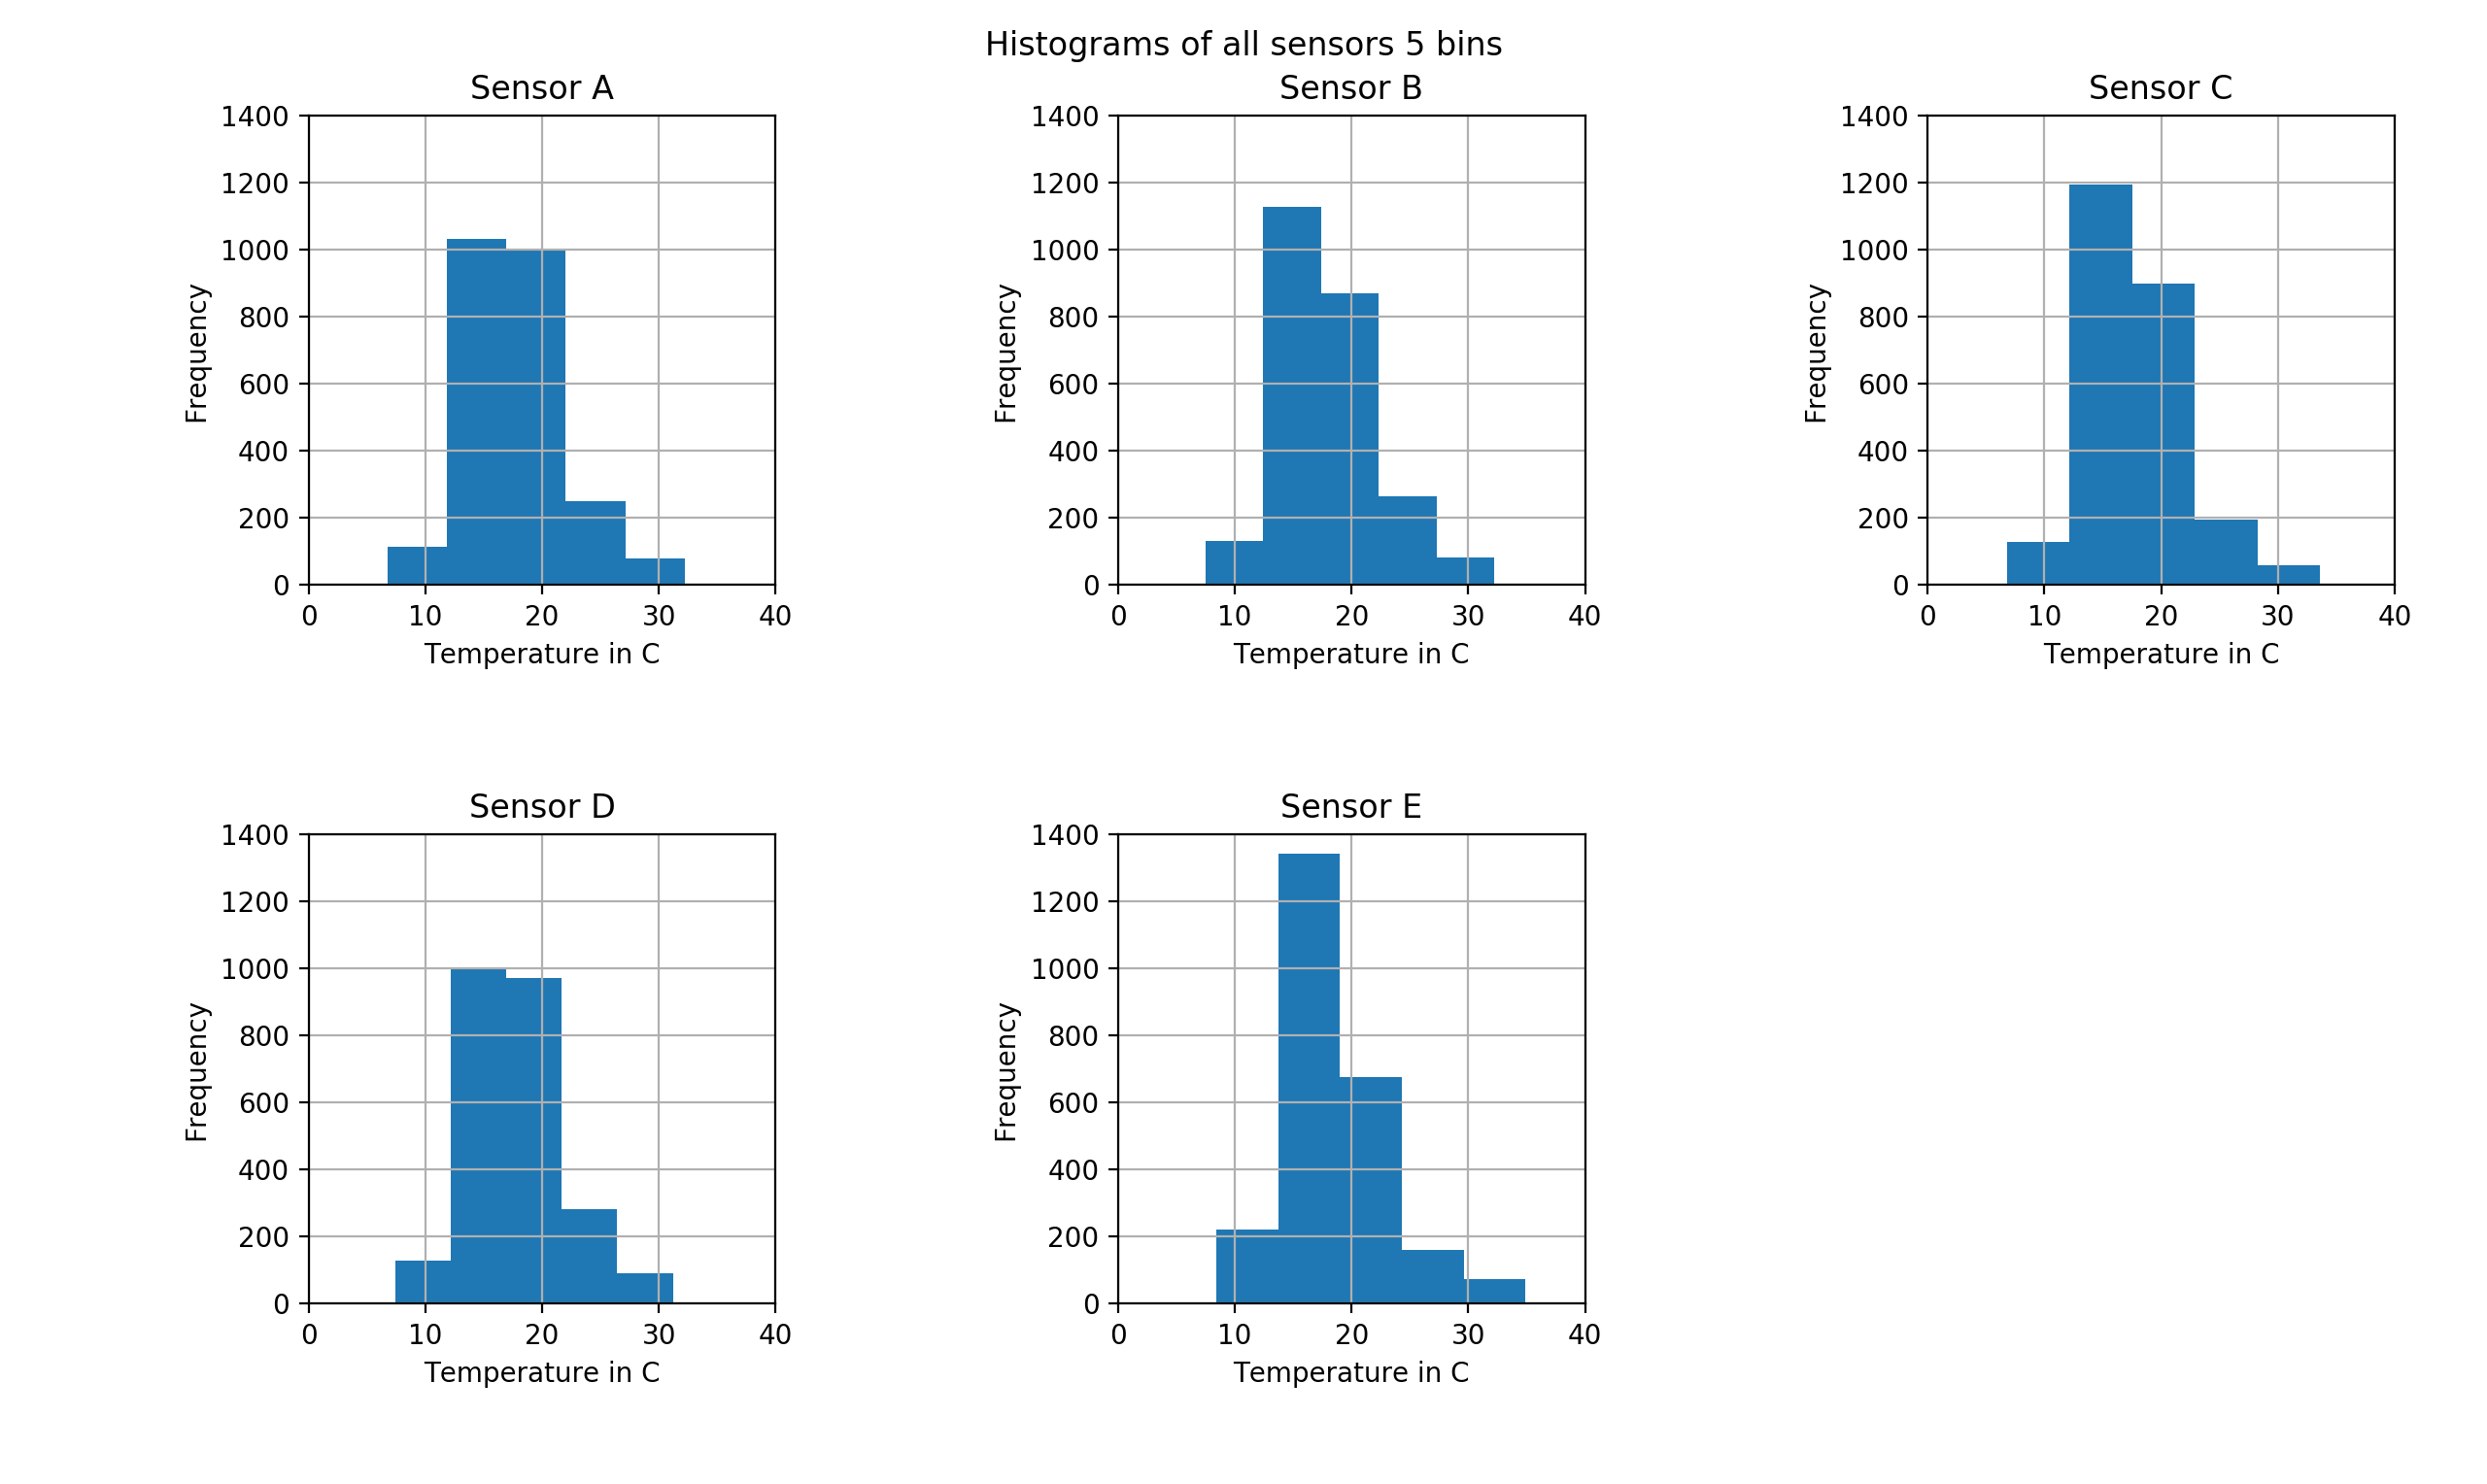
\includegraphics[width=\textwidth]{histogram_5_bins}
            \caption{Histograms of all sensors with 5 bins}
        \end{figure}

        \begin{figure}[H]
            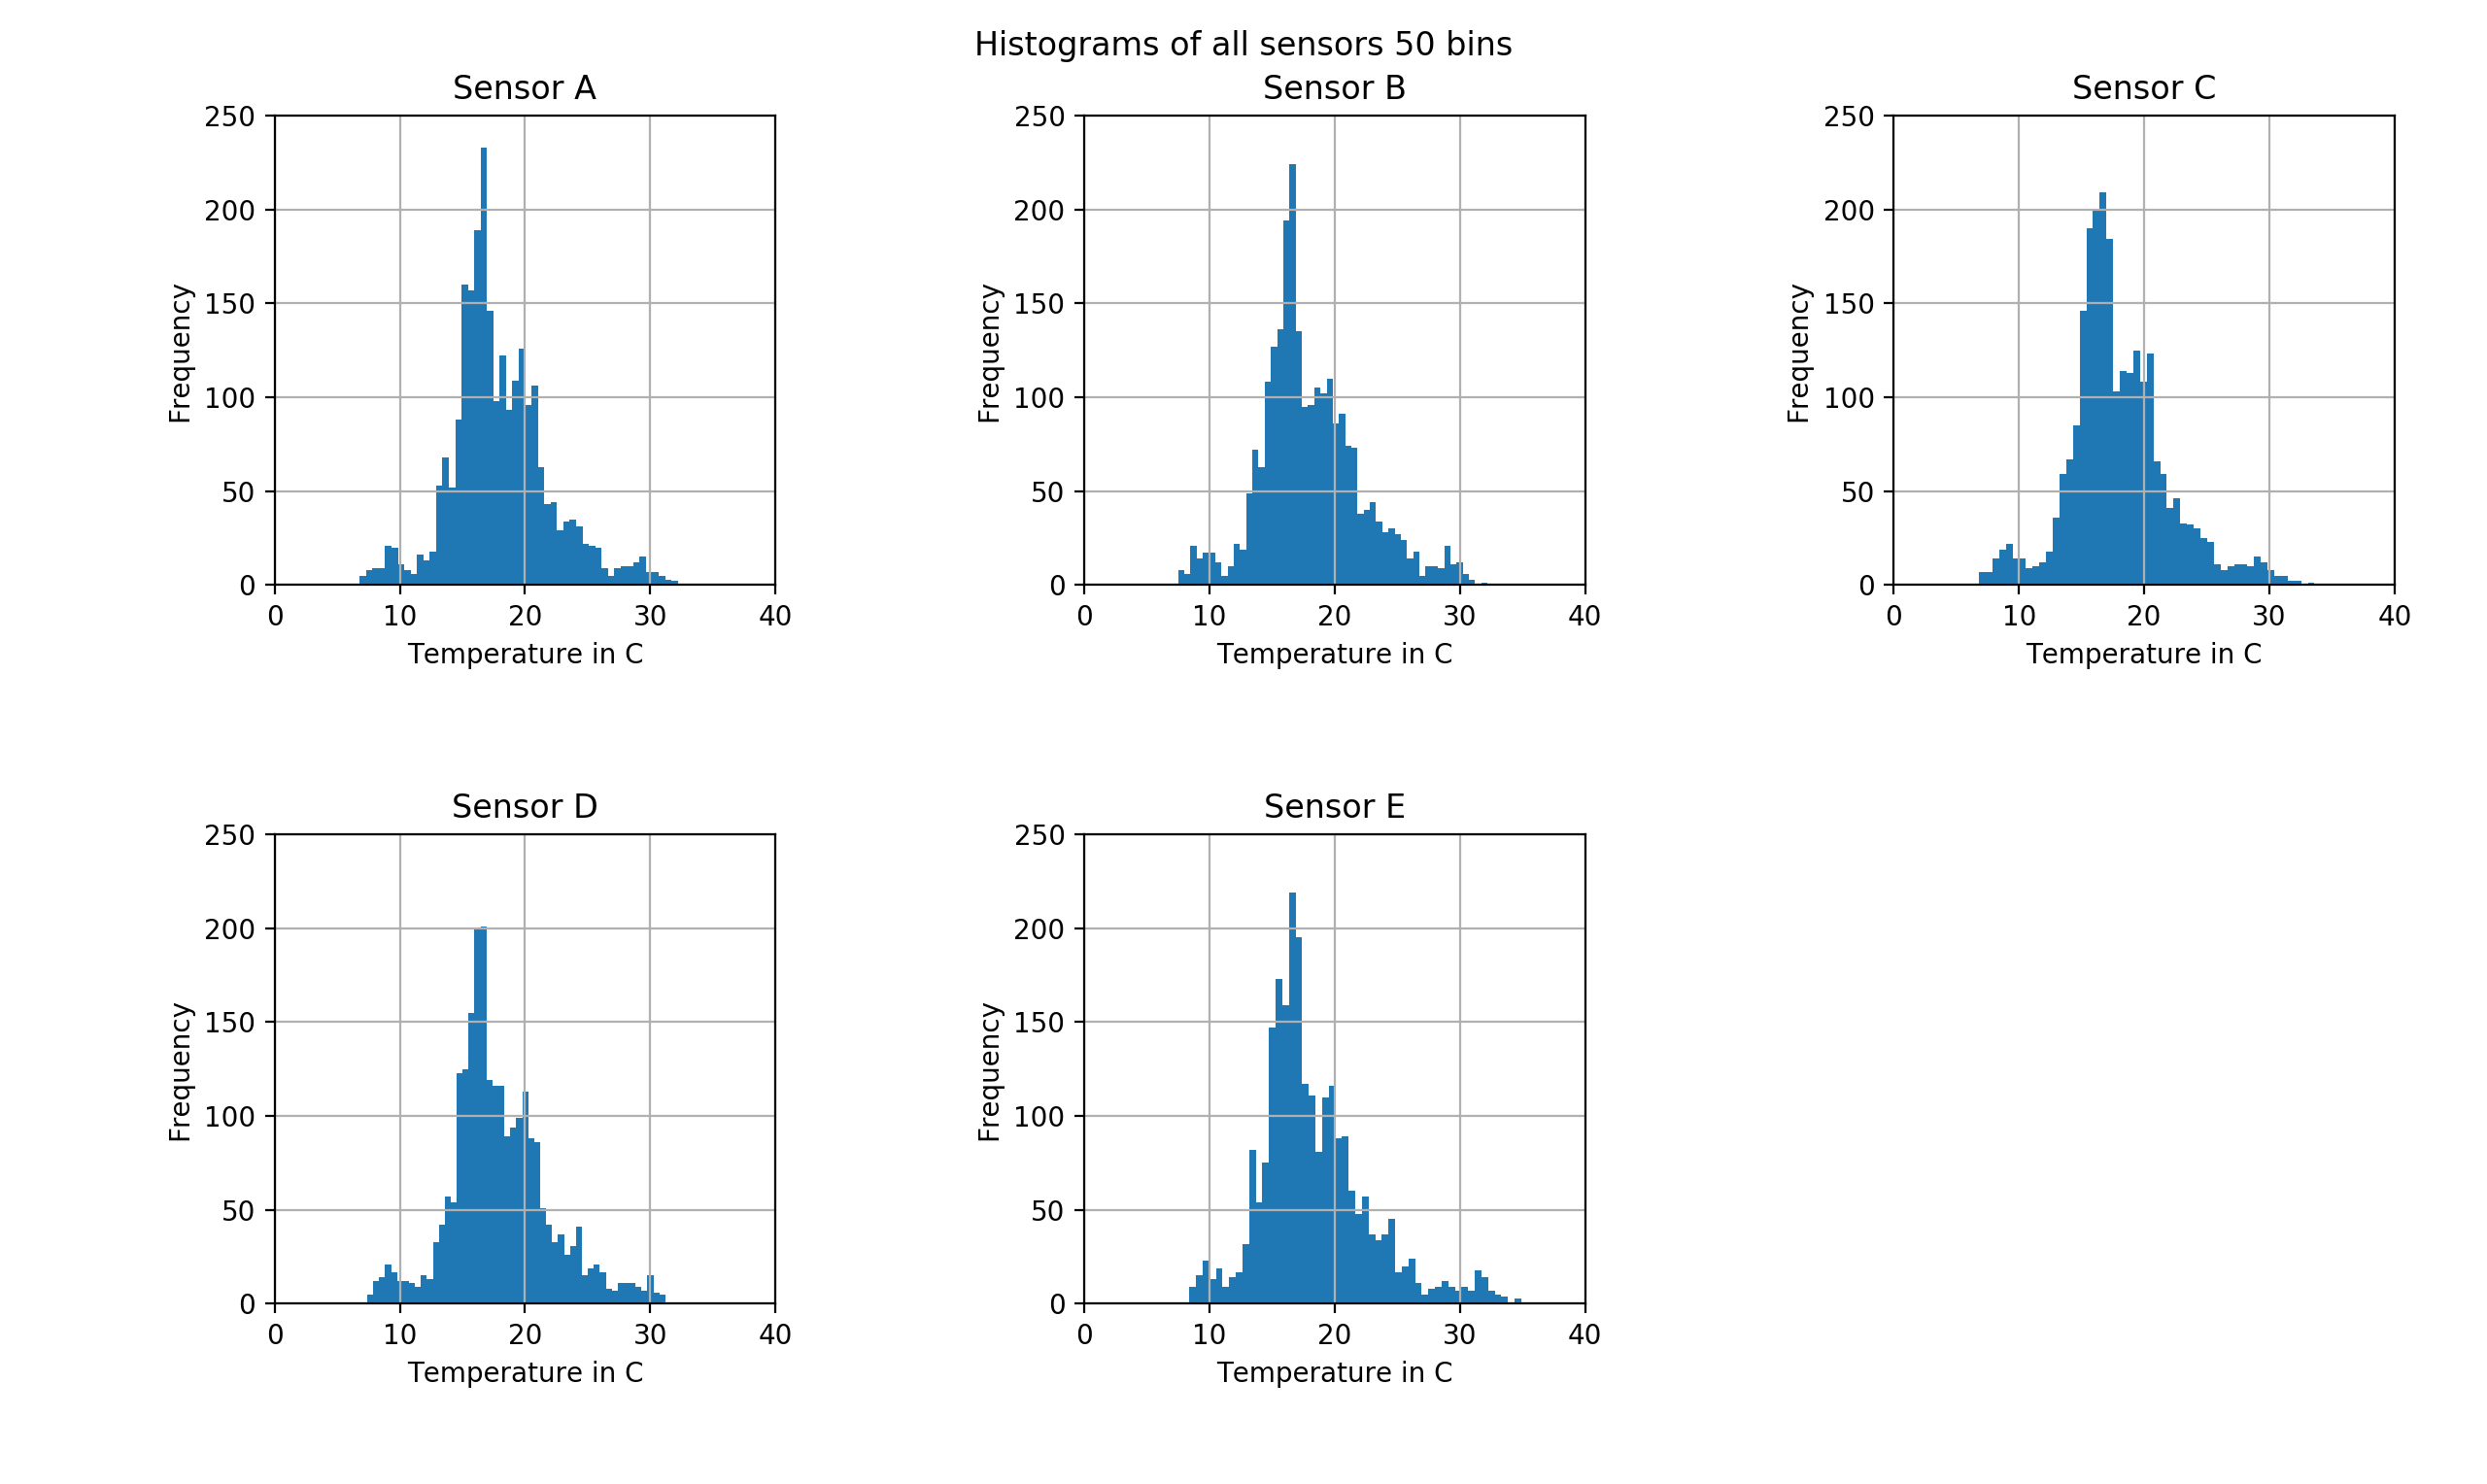
\includegraphics[width=\textwidth]{histogram_50_bins}
            \caption{Histograms of all sensors with 50 bins}
        \end{figure}
        
        In figures 1 and 2, the histograms of the temperature of the five sensors are displayed.
        As can be seen, there is a significant difference between the figures due to the bin sizes.
        Figure 2 with binsize 50 is much more detailed, which makes this figure more useful for analysation.
        The binsize calculated with Rice's rule is approximately in the middle between 5 and 50. 
        Rice's rule \ 2 * $\sqrt[3]{N}$ \ with \ N = 2474 \ gives 27 as a number of bins. 



    \subsection{Frequency polygons}
        \begin{figure}[H]
            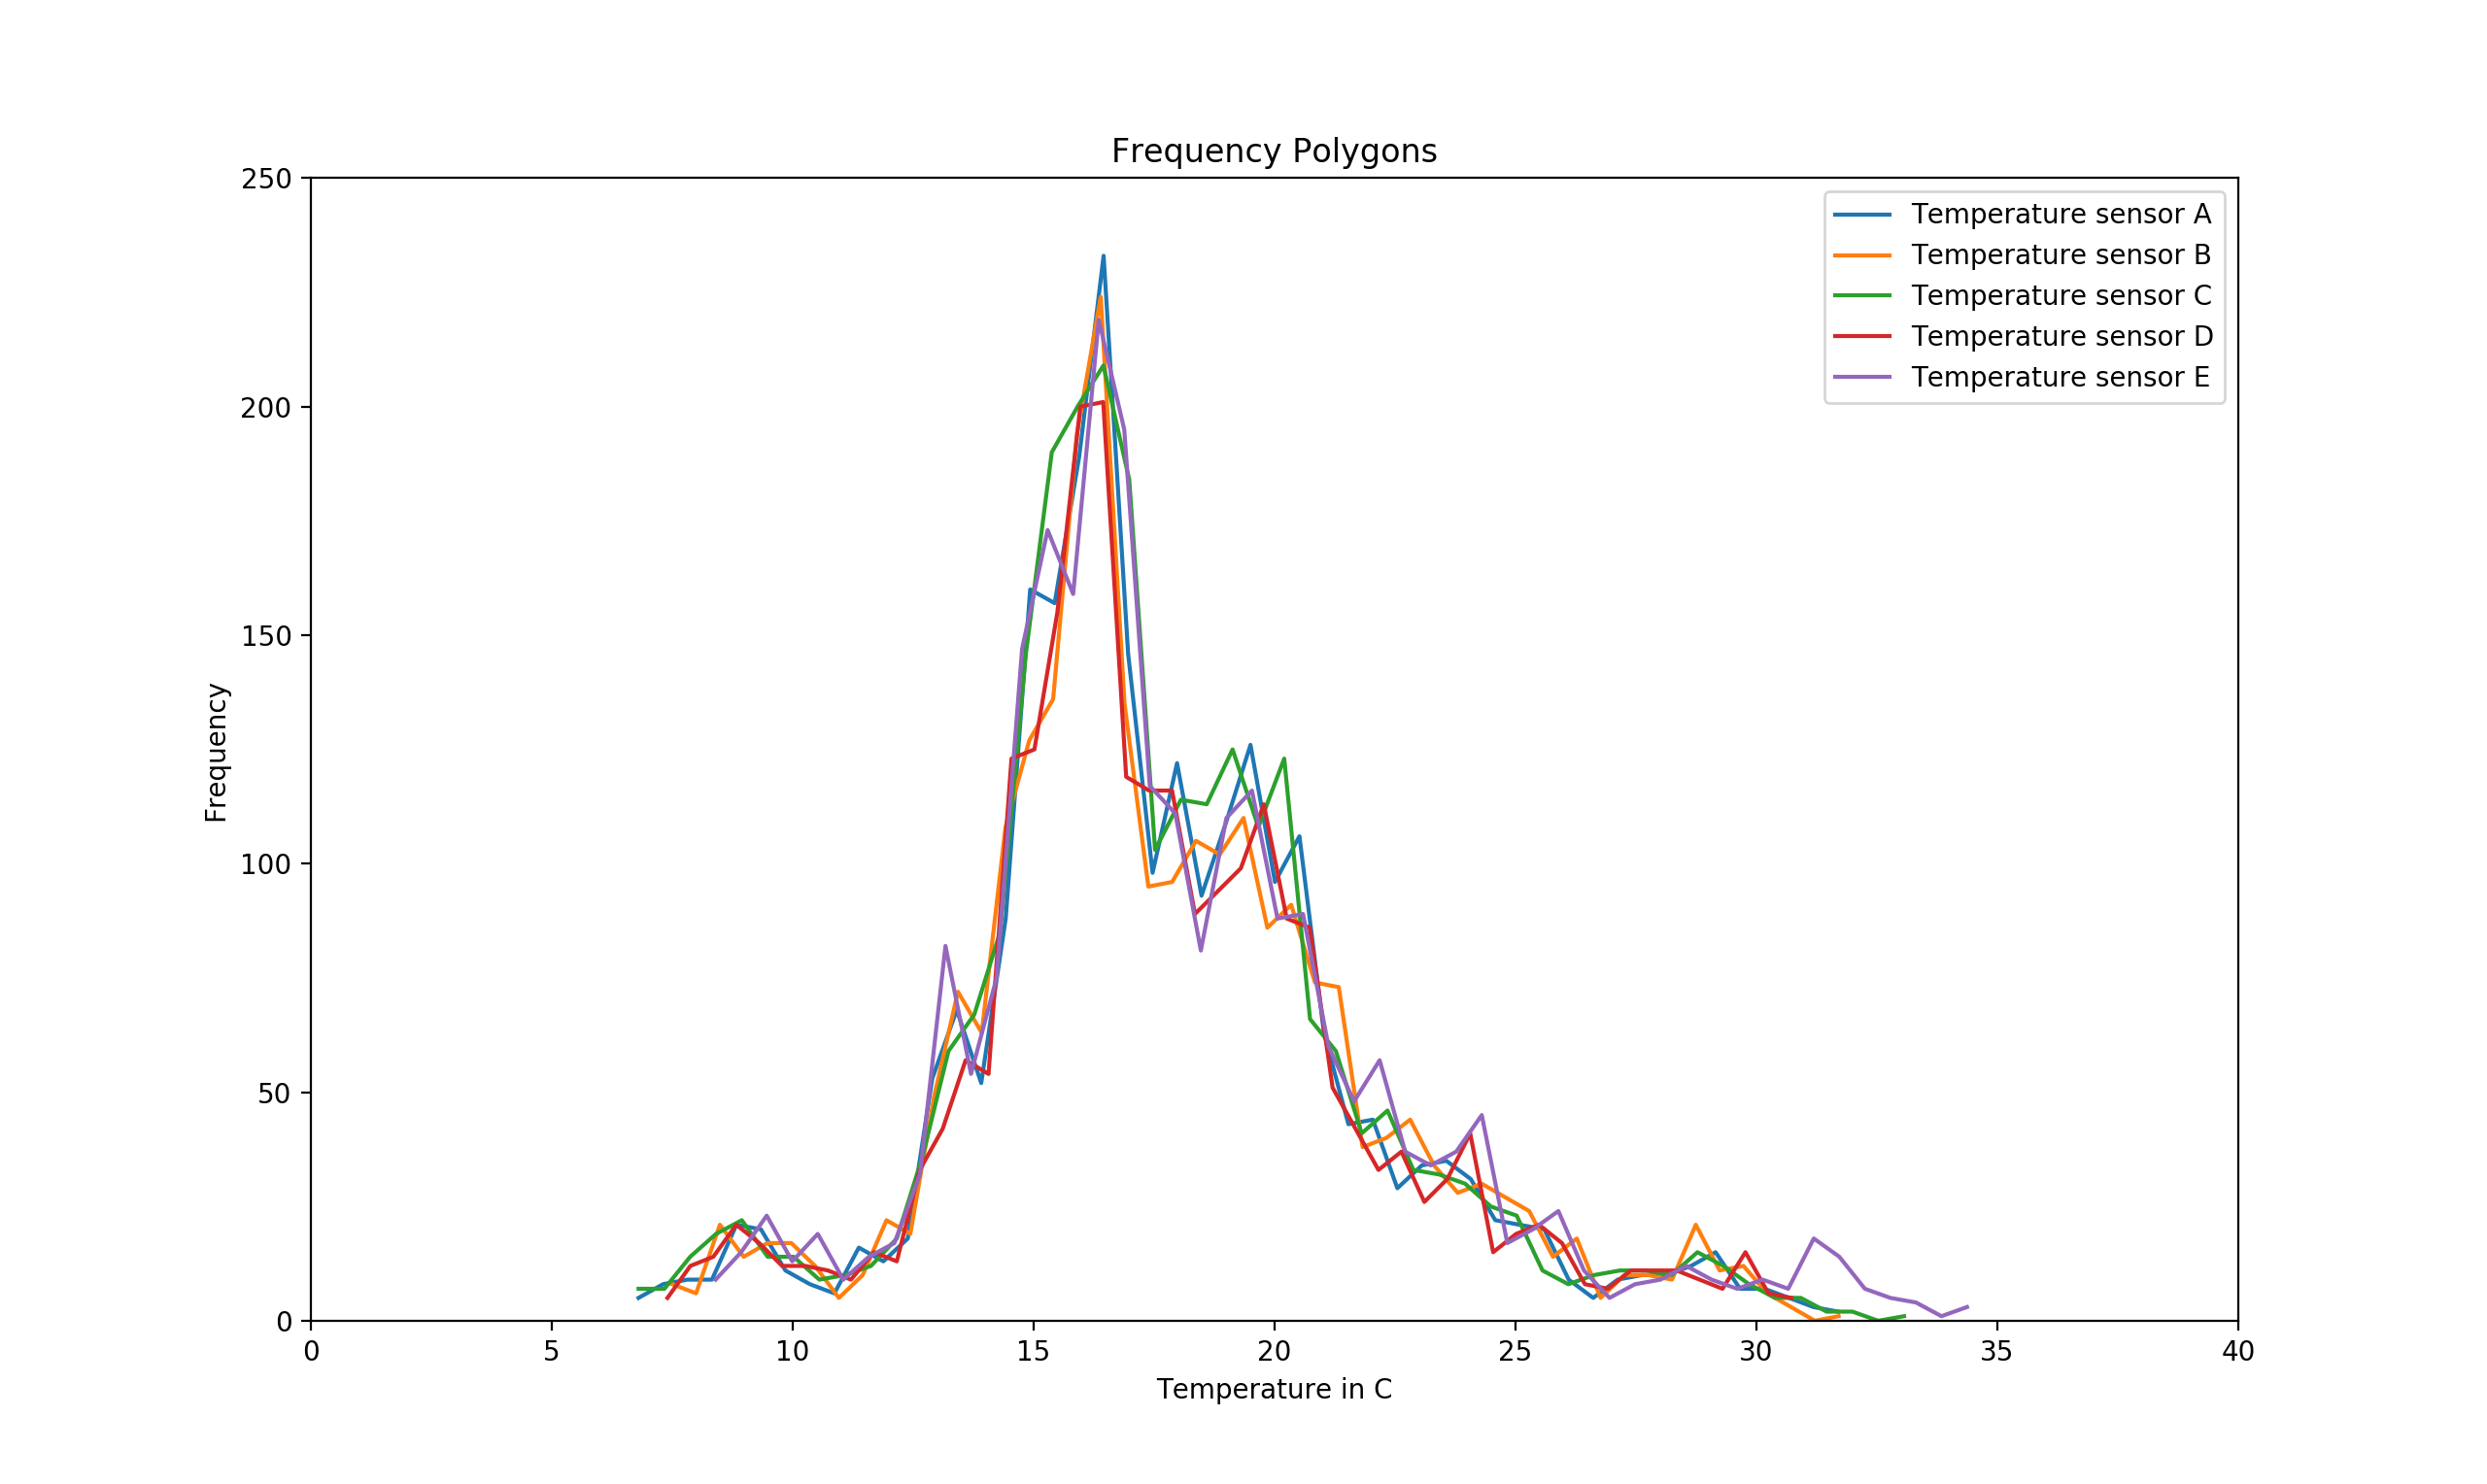
\includegraphics[width=\textwidth]{frequency_polygons_temp}
            \caption{Frequency polygon of all sensors for the variable Temperature}
        \end{figure}
            

    \subsection{Boxplots}
        
        \begin{figure}[H]
            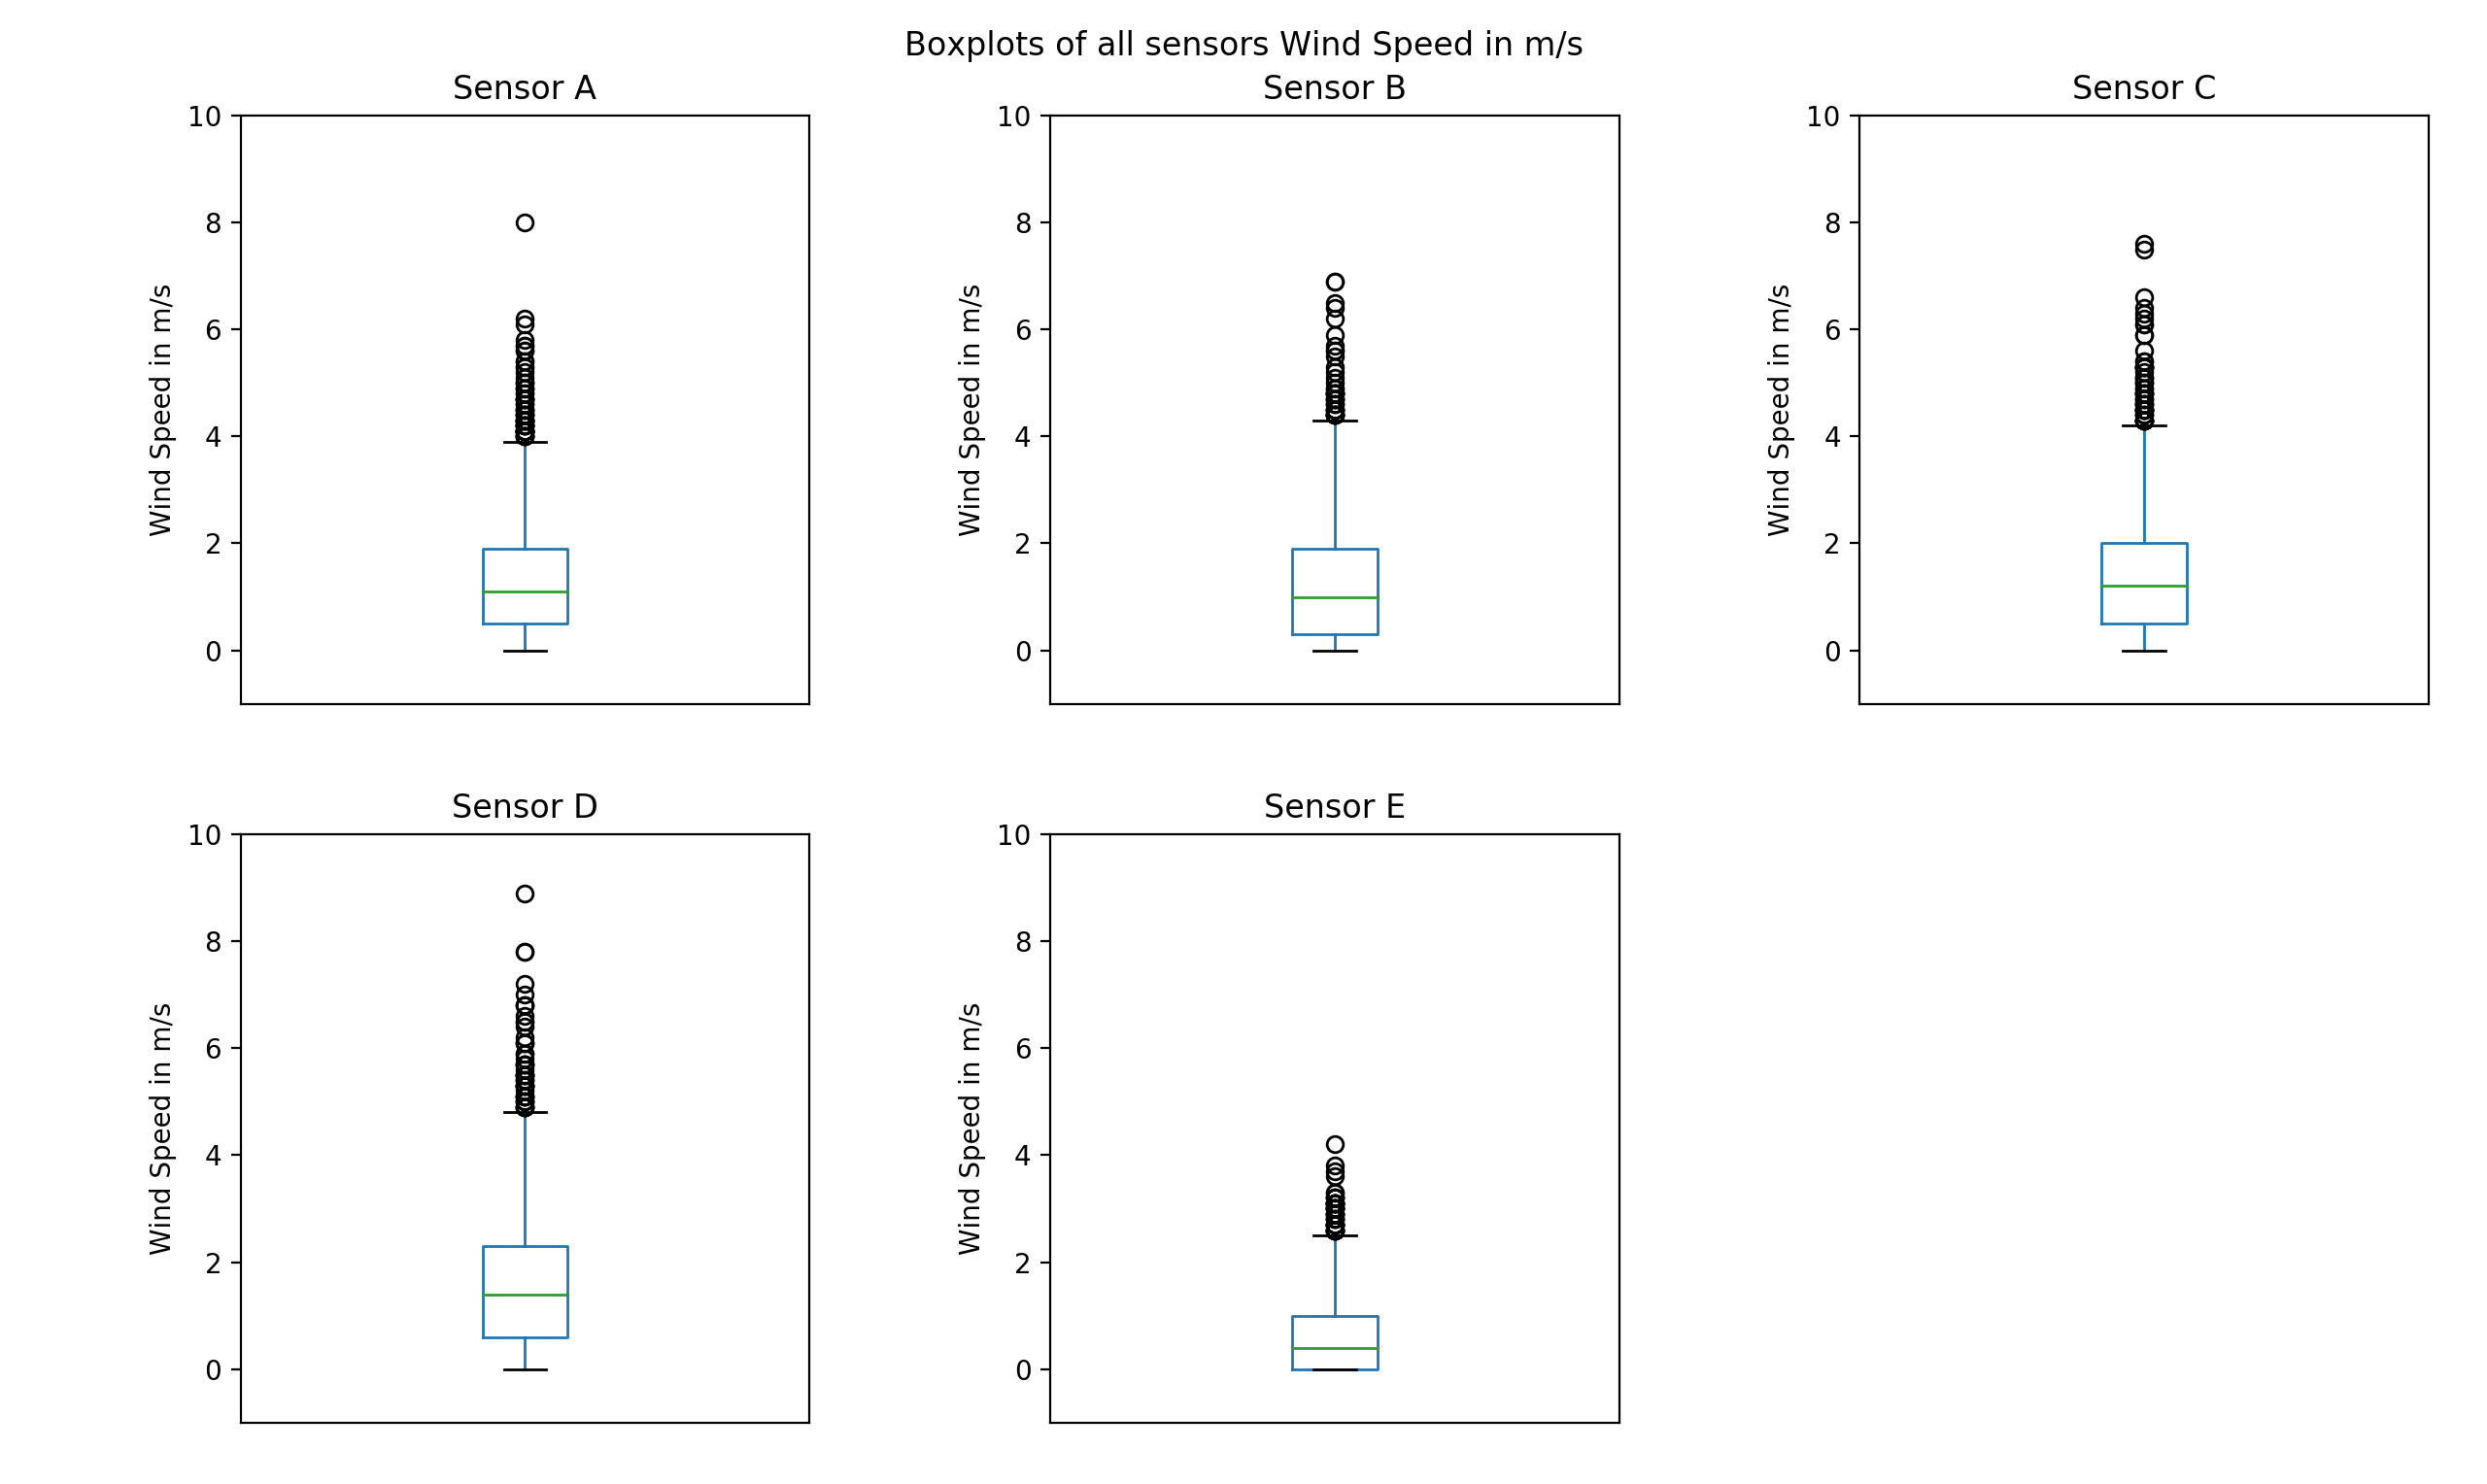
\includegraphics[width=\textwidth]{boxplot_windspeed}
            \caption{Boxplots of all sensors for the variable Wind Speed}
        \end{figure}
        
        \begin{figure}[H]
            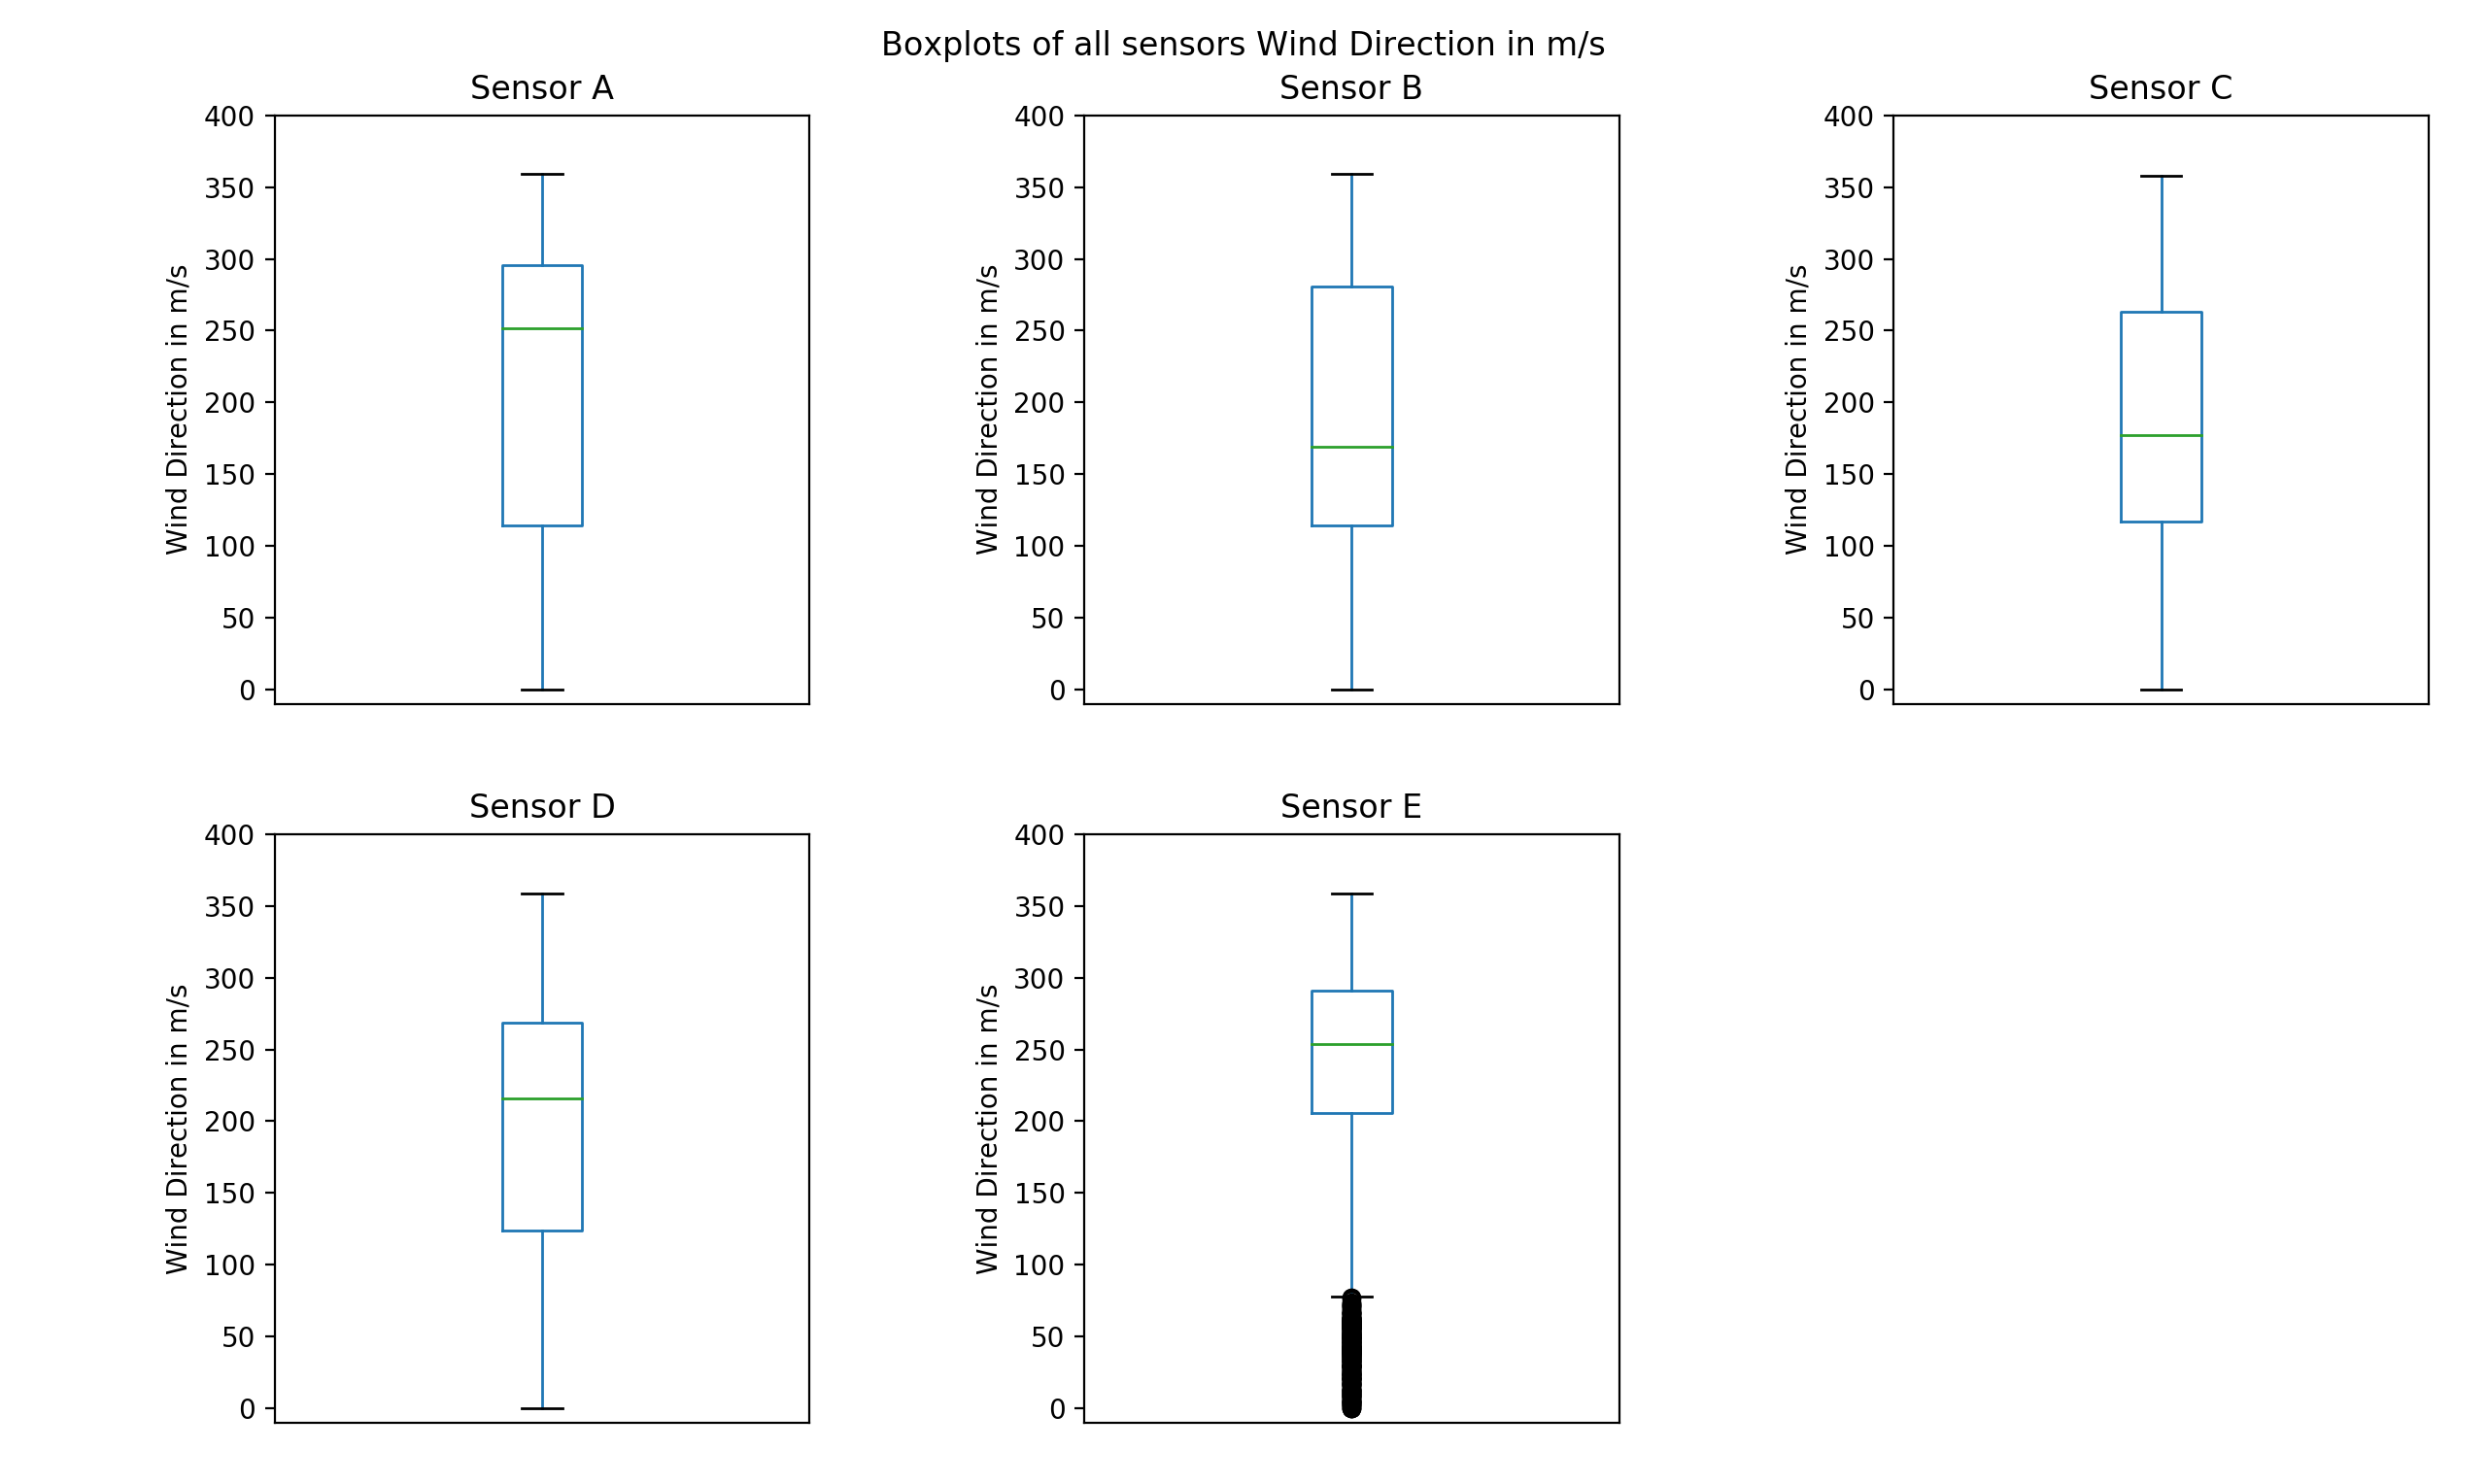
\includegraphics[width=\textwidth]{boxplot_winddirection}
            \caption{Boxplots of all sensors for the variable Wind Direction}
        \end{figure}
        
        \begin{figure}[H]
            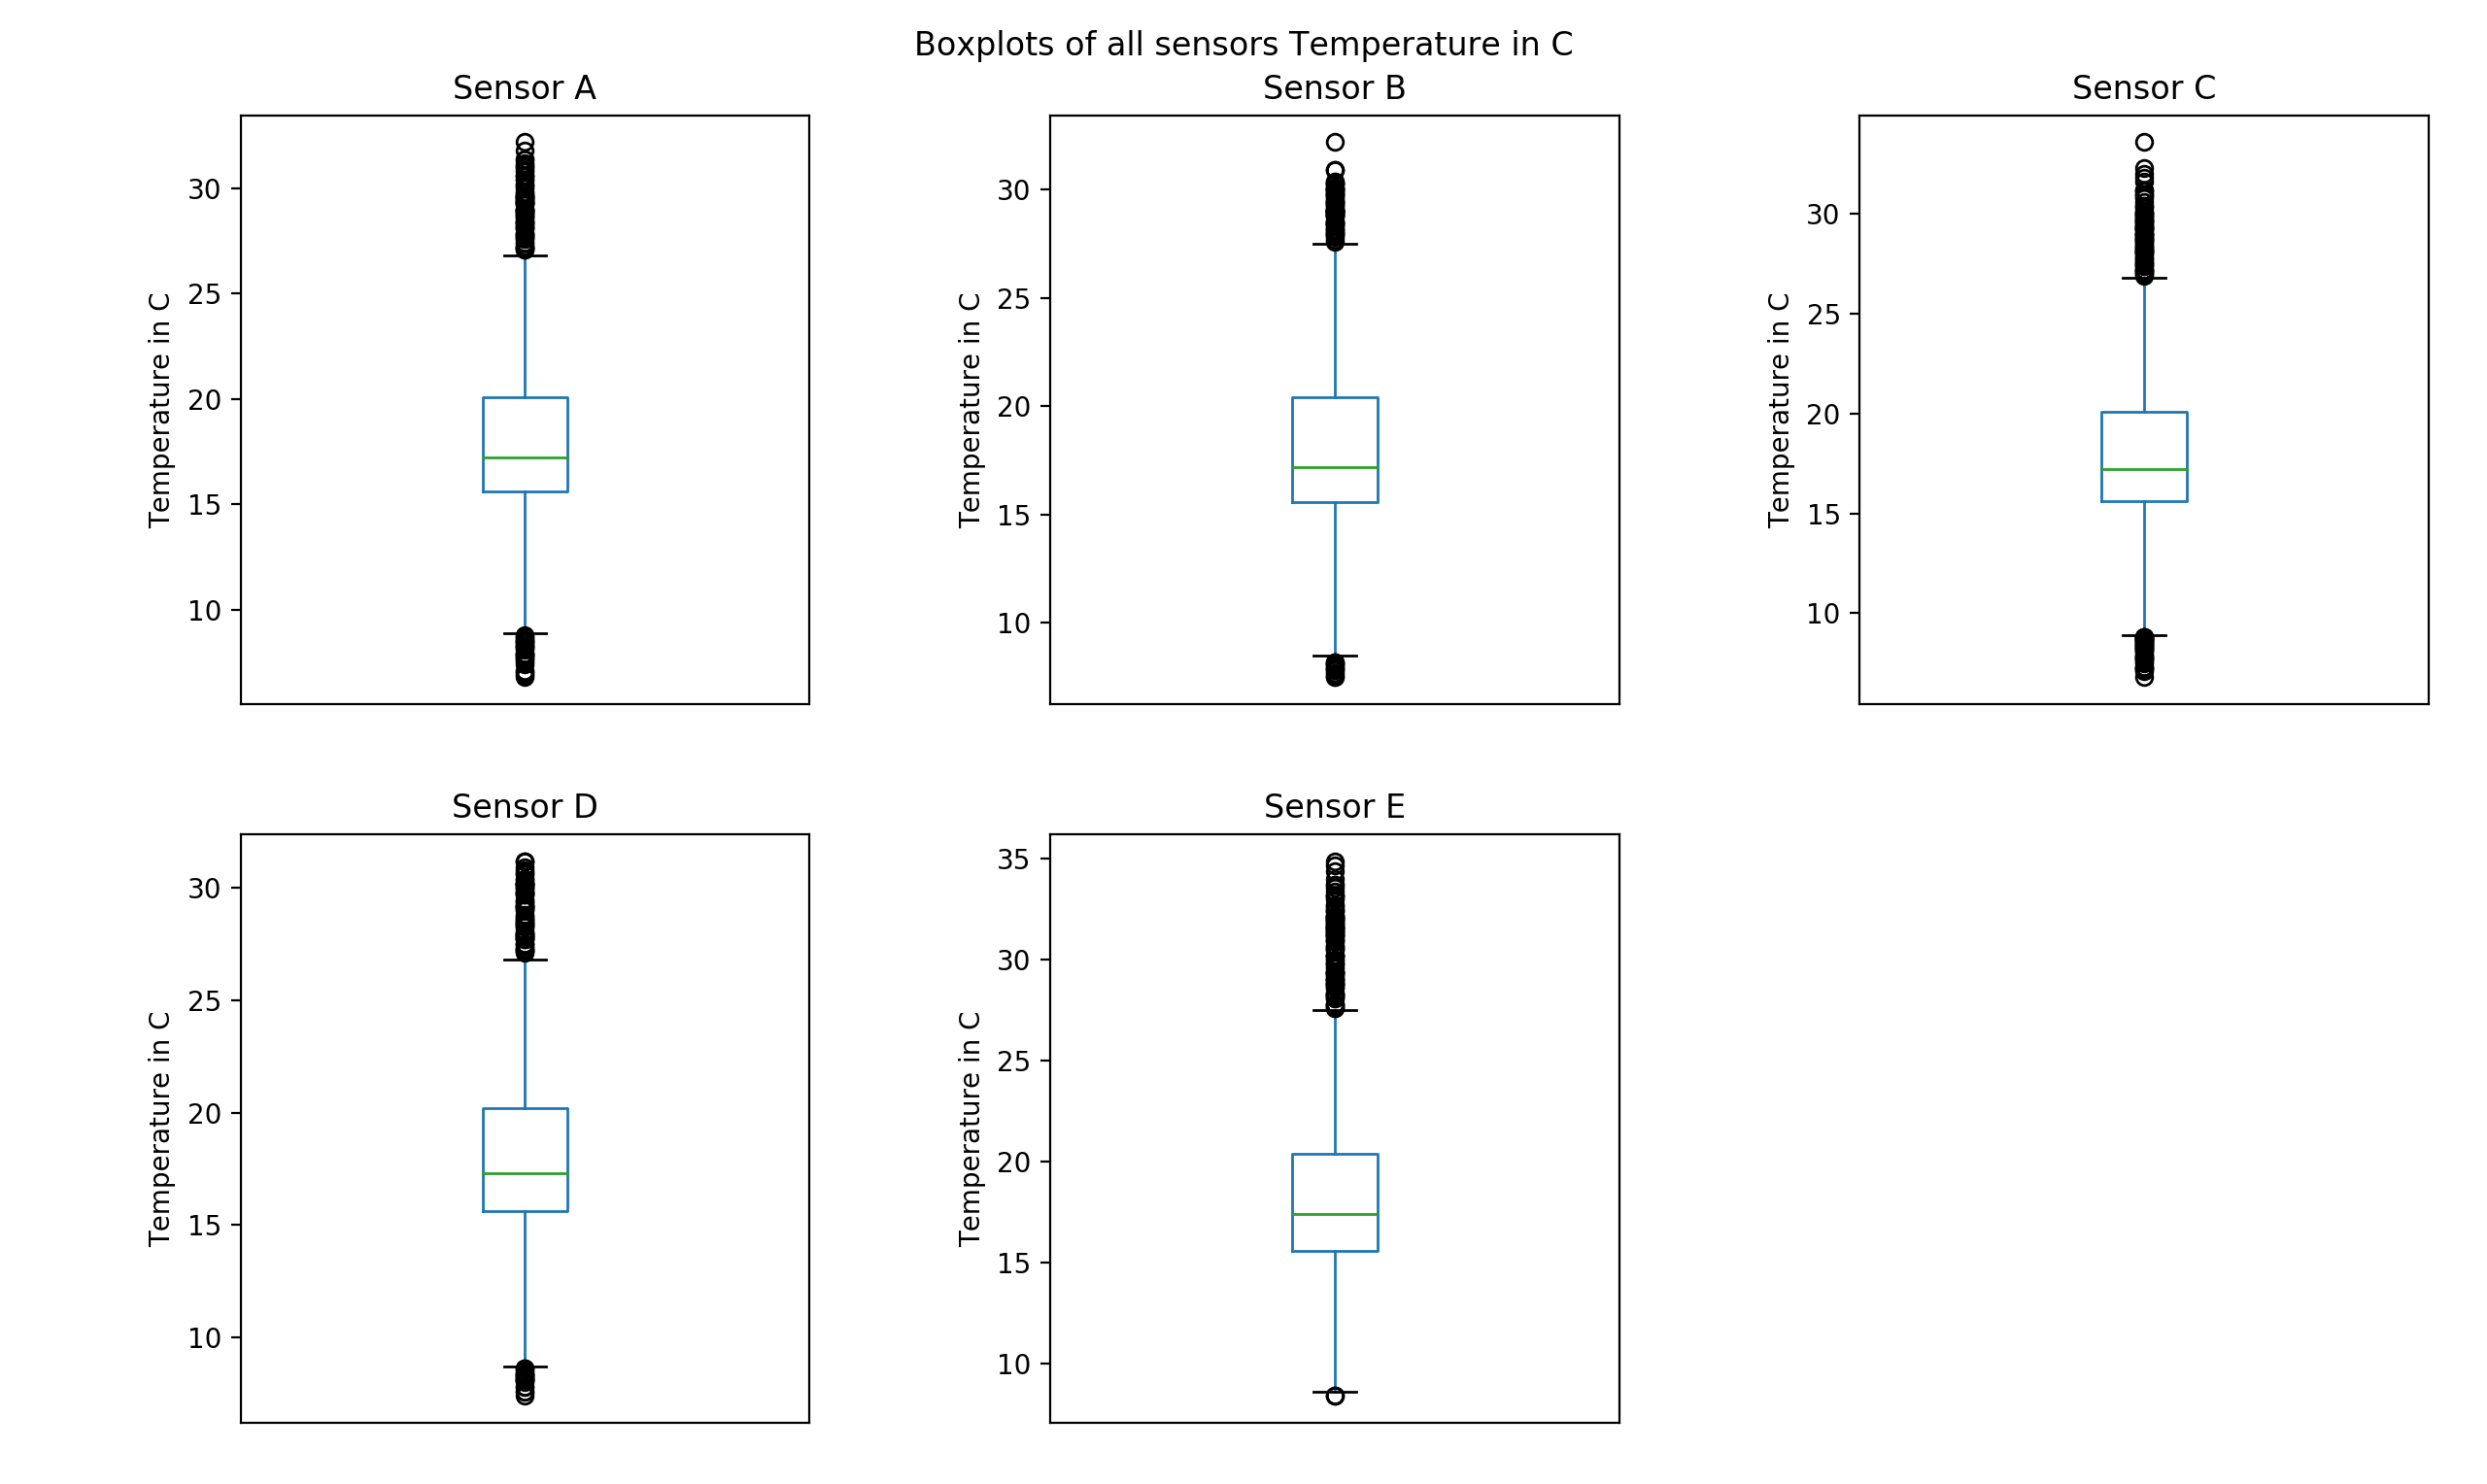
\includegraphics[width=\textwidth]{boxplot_temperature}
            \caption{Boxplots of all sensors for the variable Temperature}
        \end{figure}
        

\section{A2}
        \subsection{Functions Temperature}
            \begin{figure}[H]
                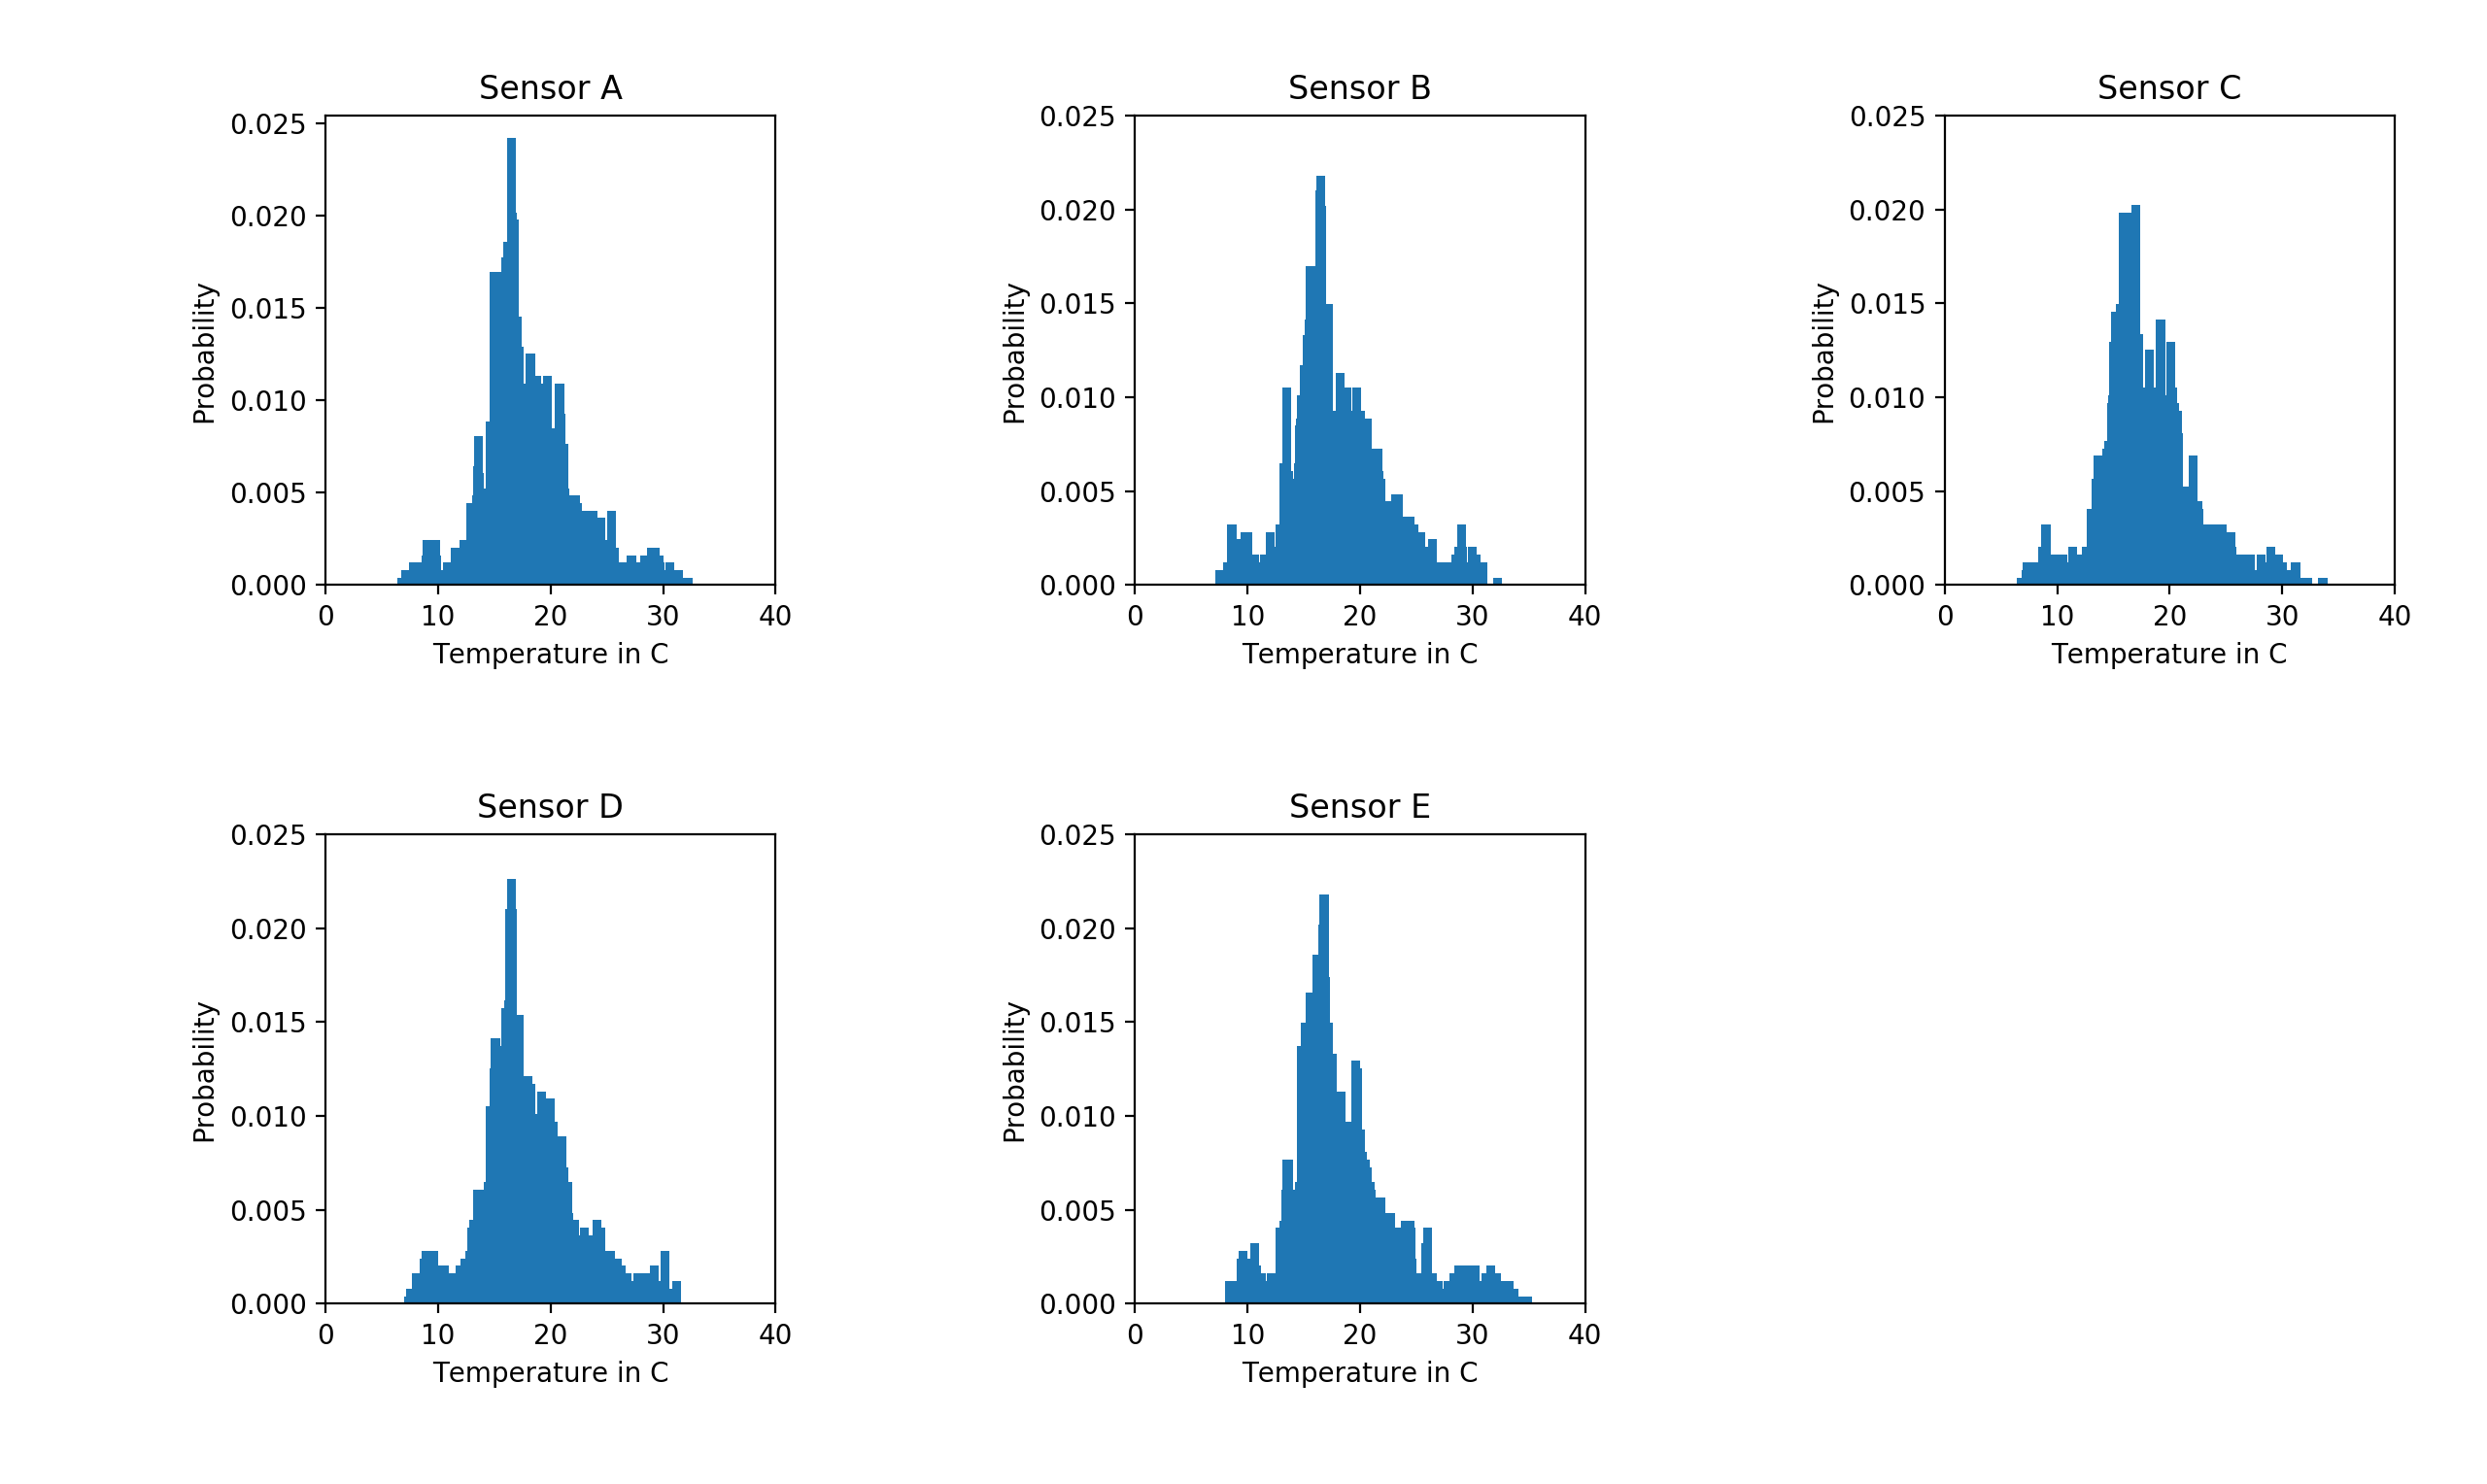
\includegraphics[width=\textwidth]{pmf_temp}
                \caption{Probability Mass Functions of Temperature for all sensors}
            \end{figure}

            \begin{figure}[H]
                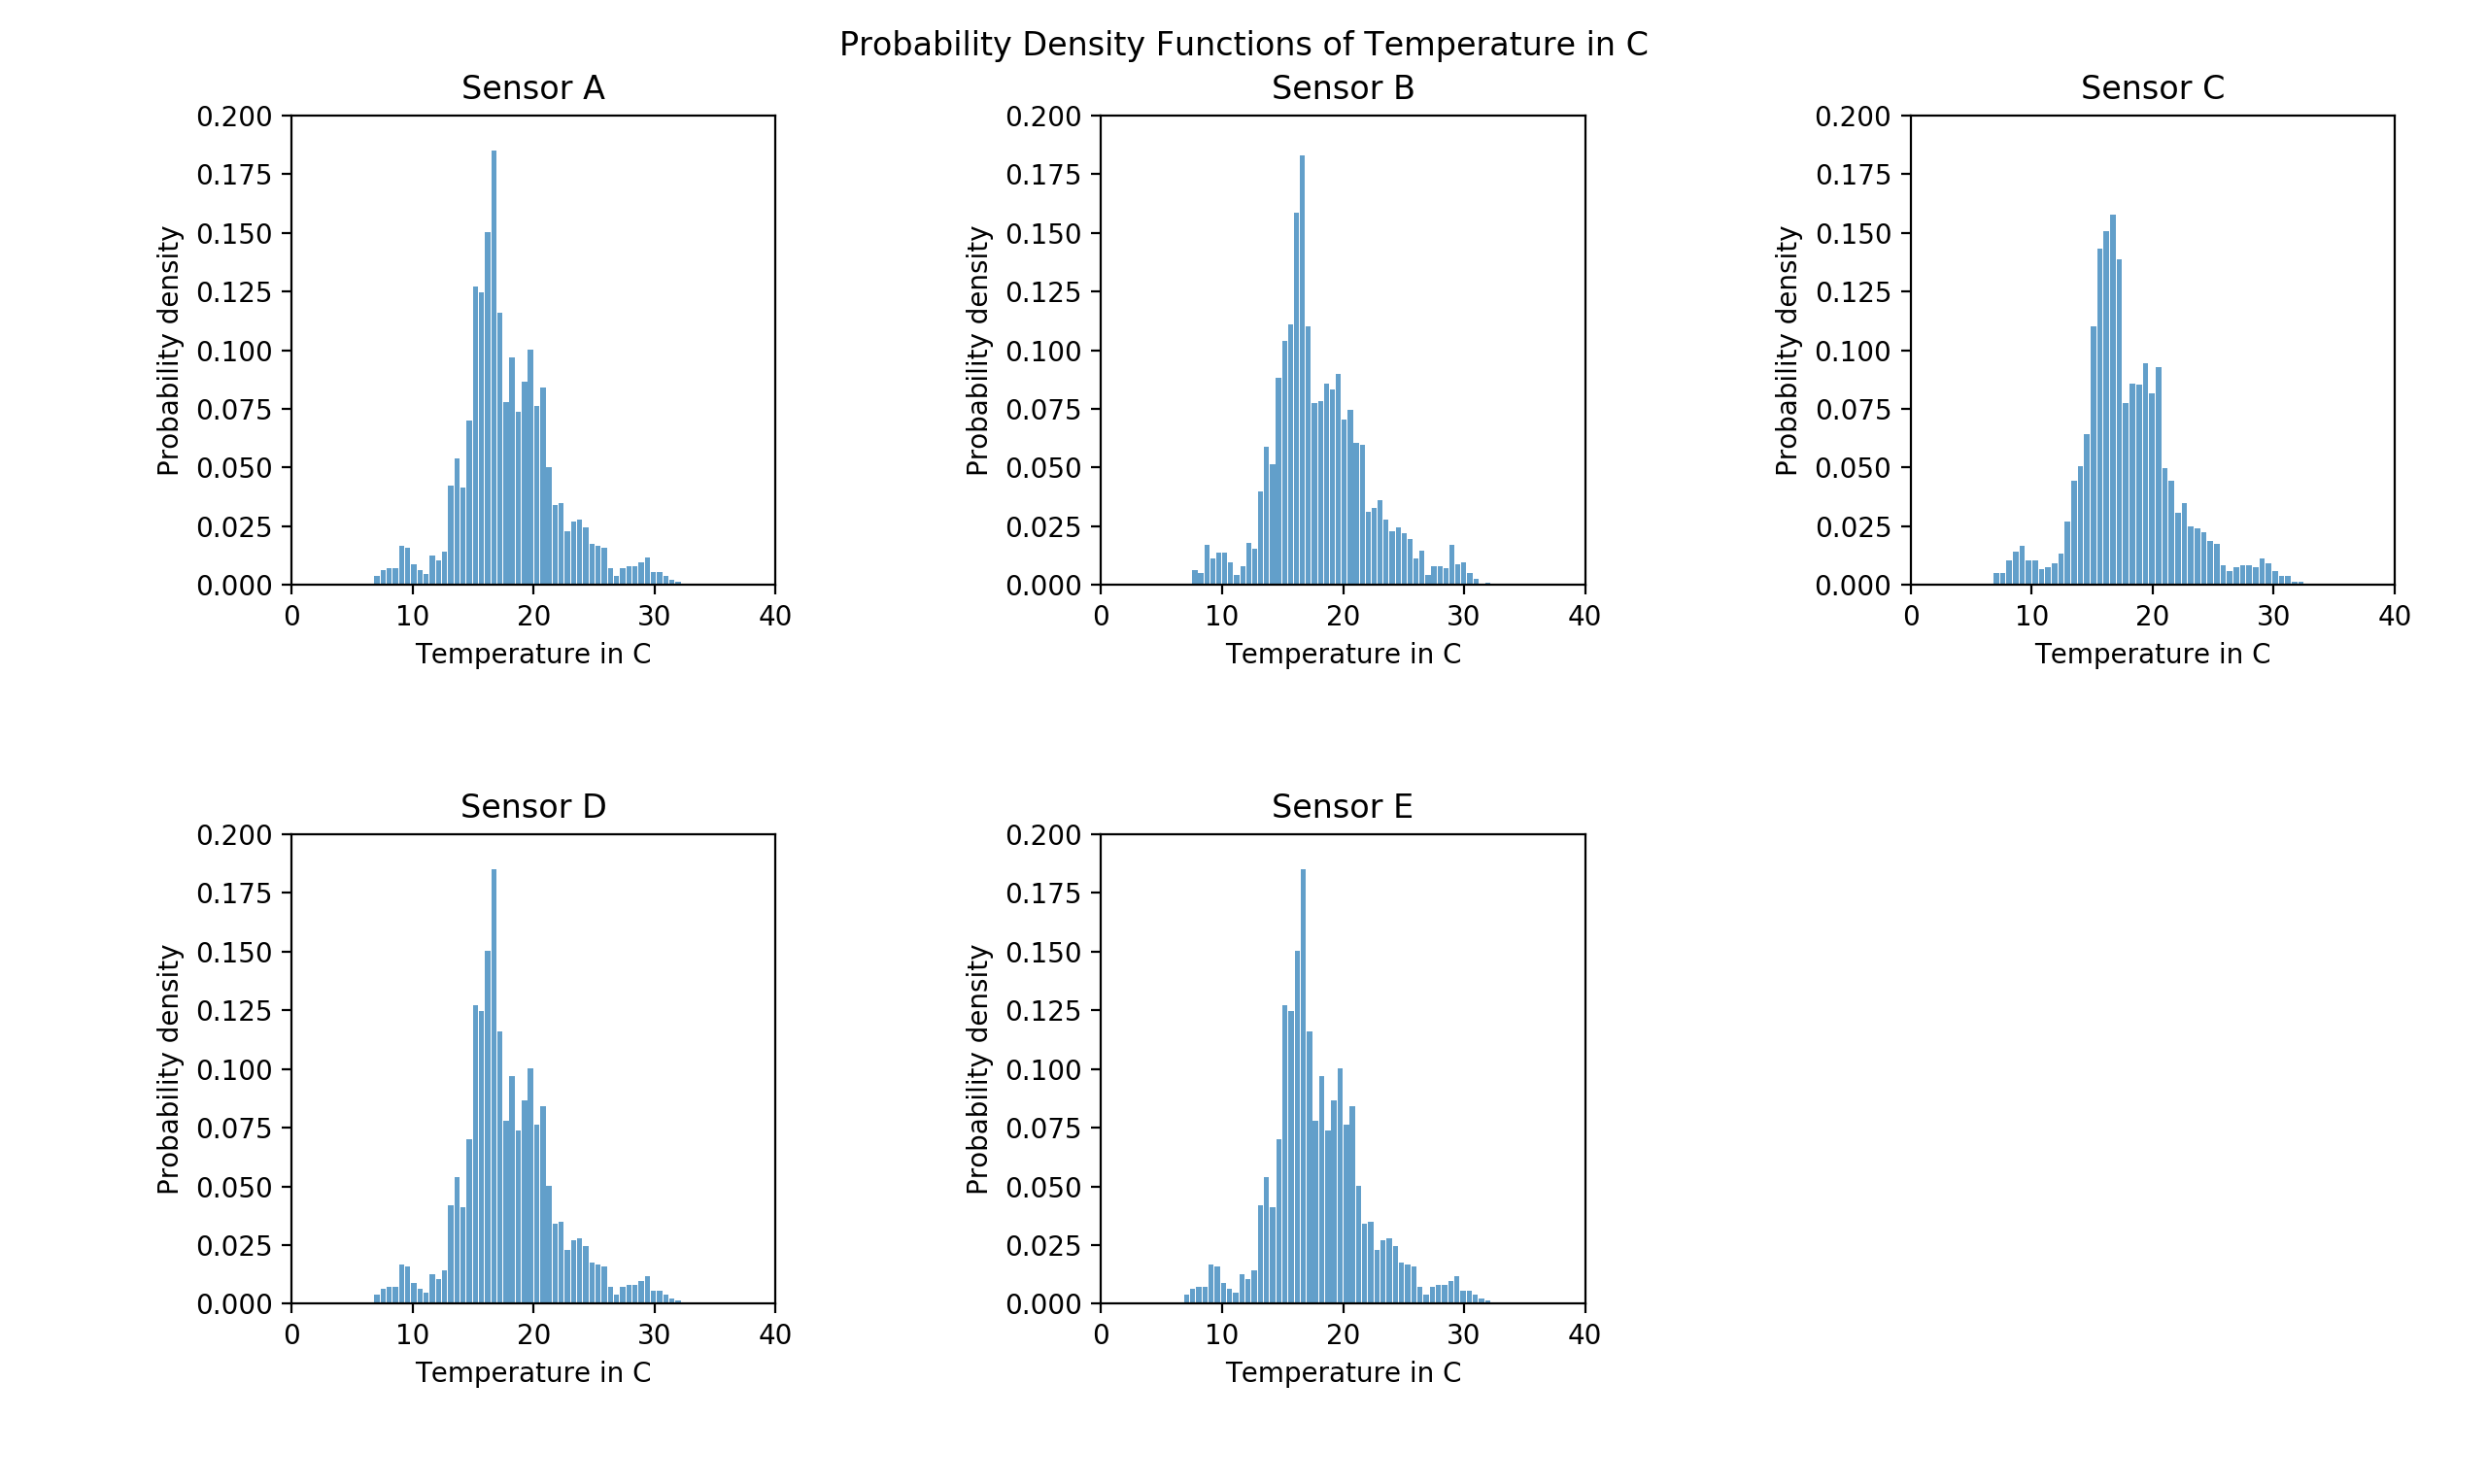
\includegraphics[width=\textwidth]{pdf_temp}
                \caption{Probability Density Functions of Temperature for all sensors}
            \end{figure}

            \begin{figure}[H]
                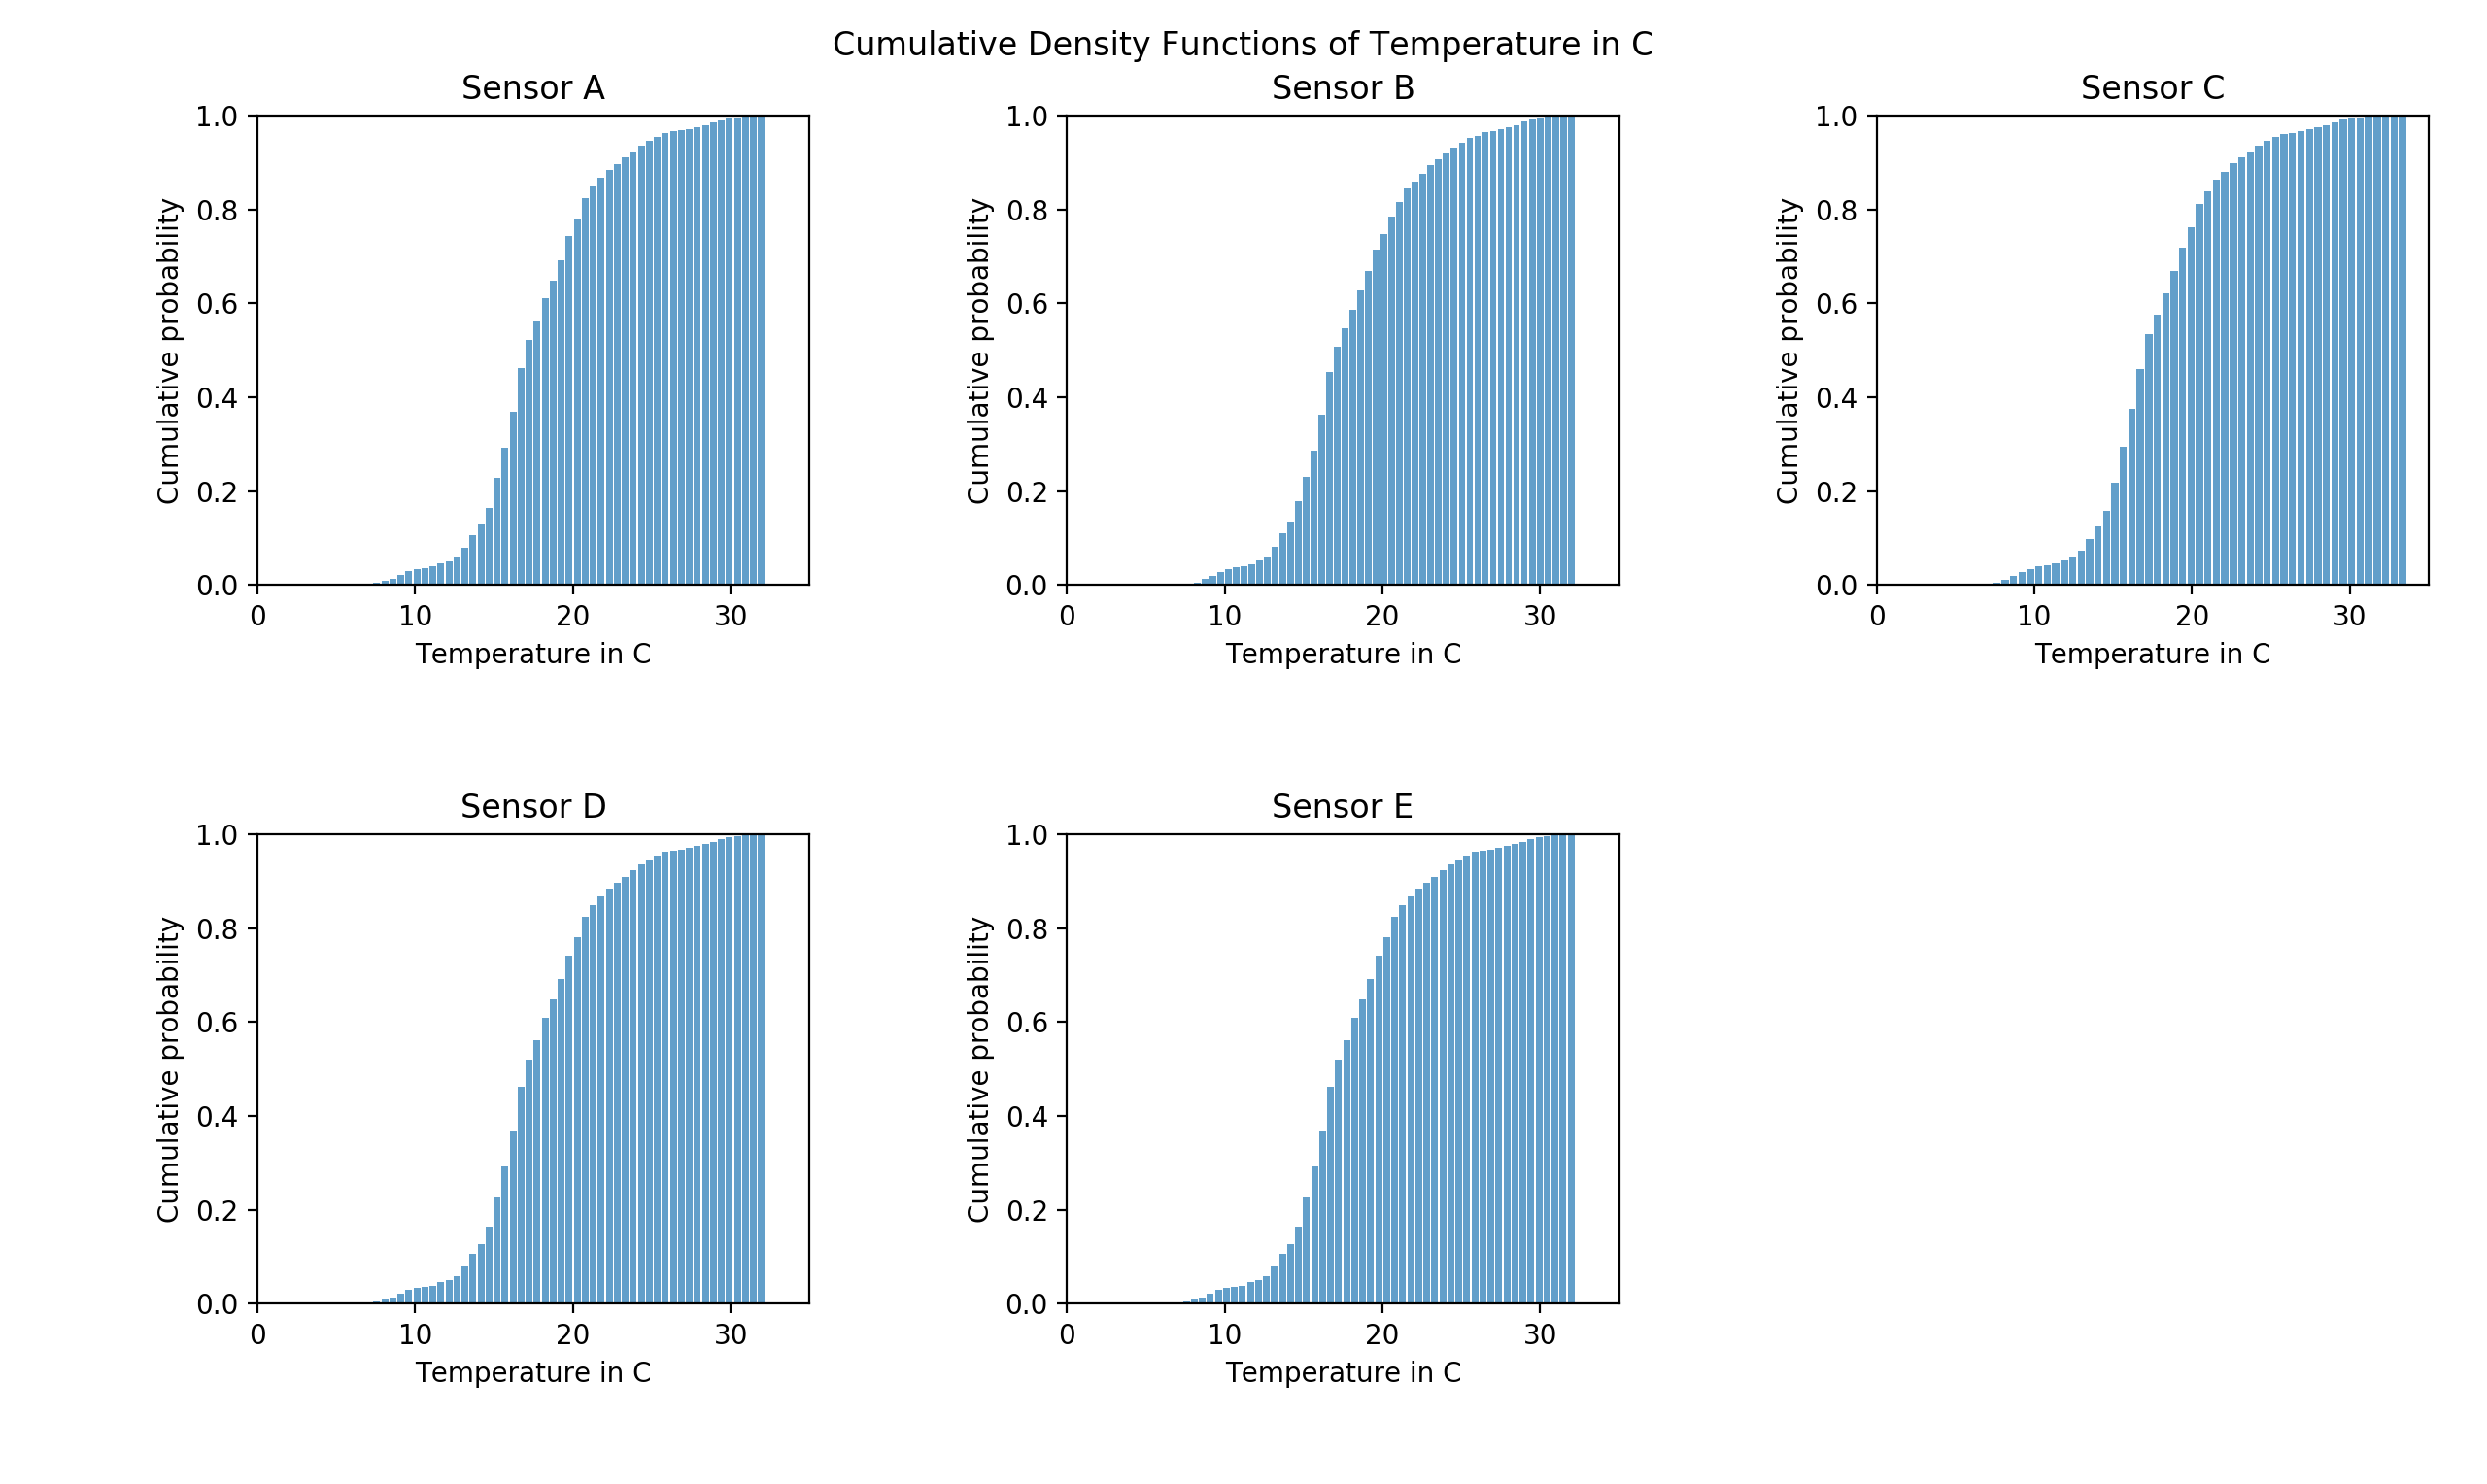
\includegraphics[width=\textwidth]{cdf_temp}
                \caption{Cumilative Density Functions of Temperature for all sensors}
            \end{figure}

        \subsection{Functions Wind Speed}
            \begin{figure}[H]
                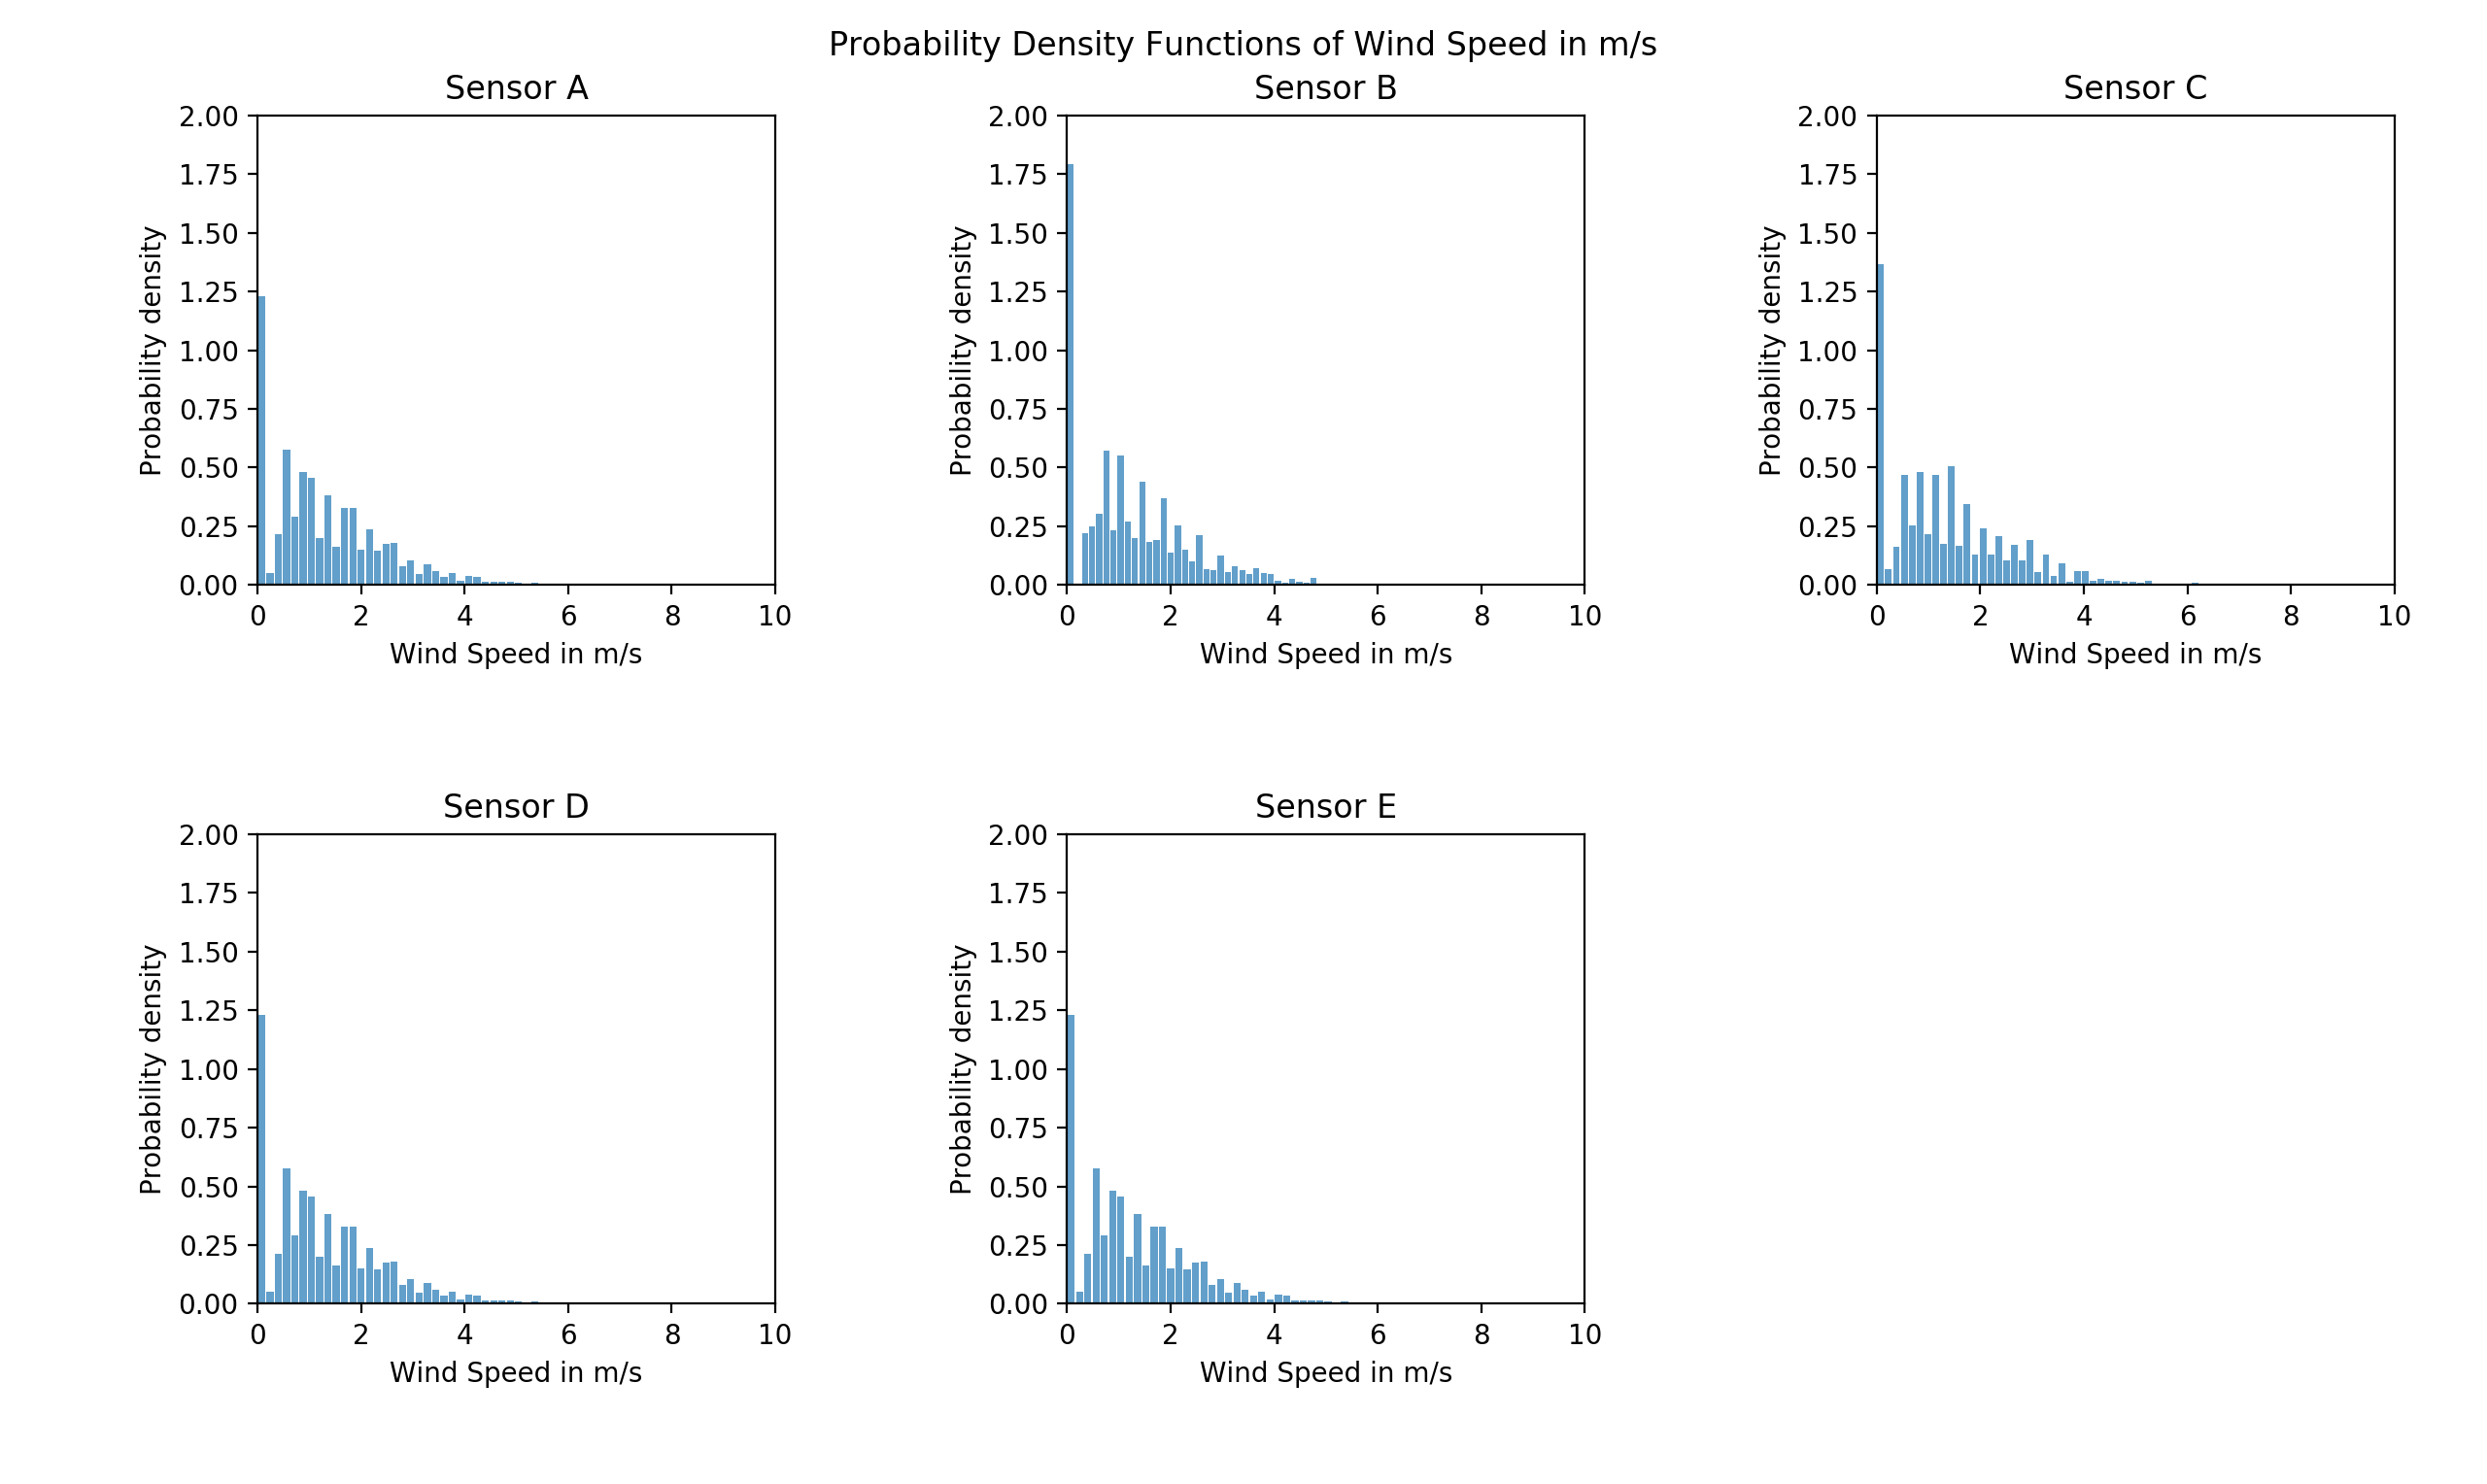
\includegraphics[width=\textwidth]{pdf_windspeed}
                \caption{Probability Density Functions of Wind Speed for all sensors}
            \end{figure}

            \begin{figure}[H]
                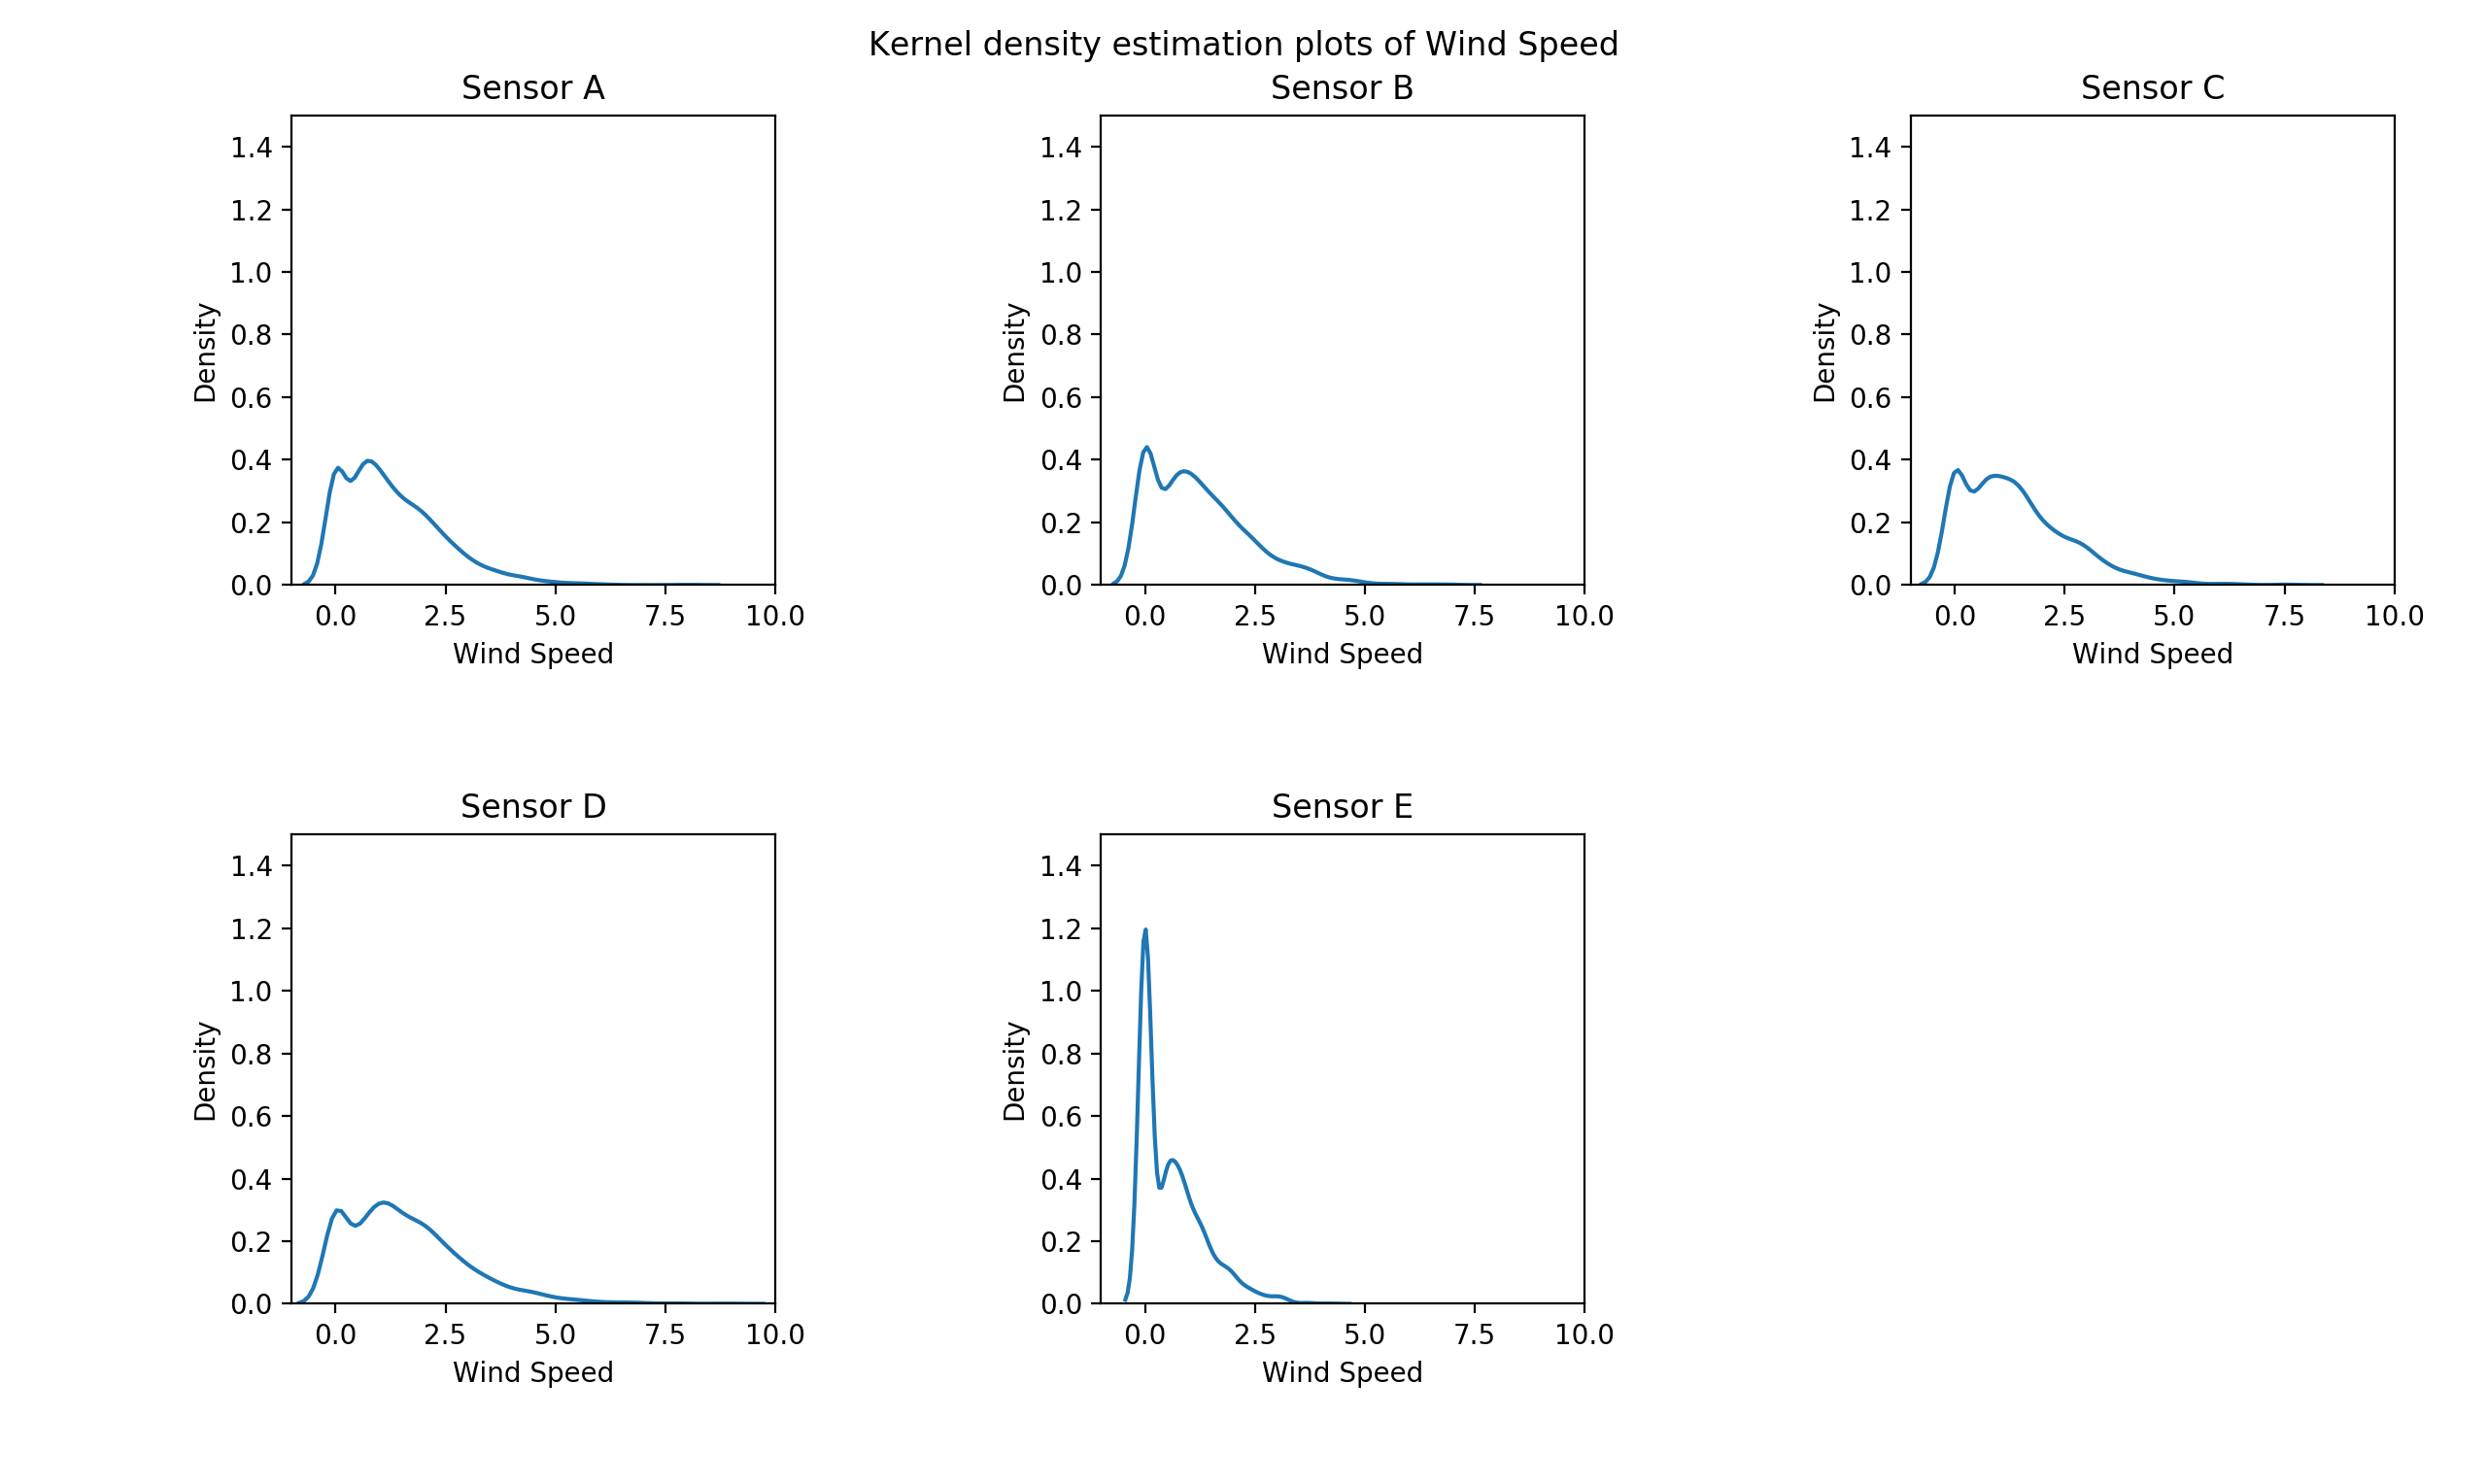
\includegraphics[width=\textwidth]{kde_windspeed}
                \caption{Kernel Density Estimation of Wind Speed for all sensors}
            \end{figure}



\section{A3}
    \begin{figure}[H]
        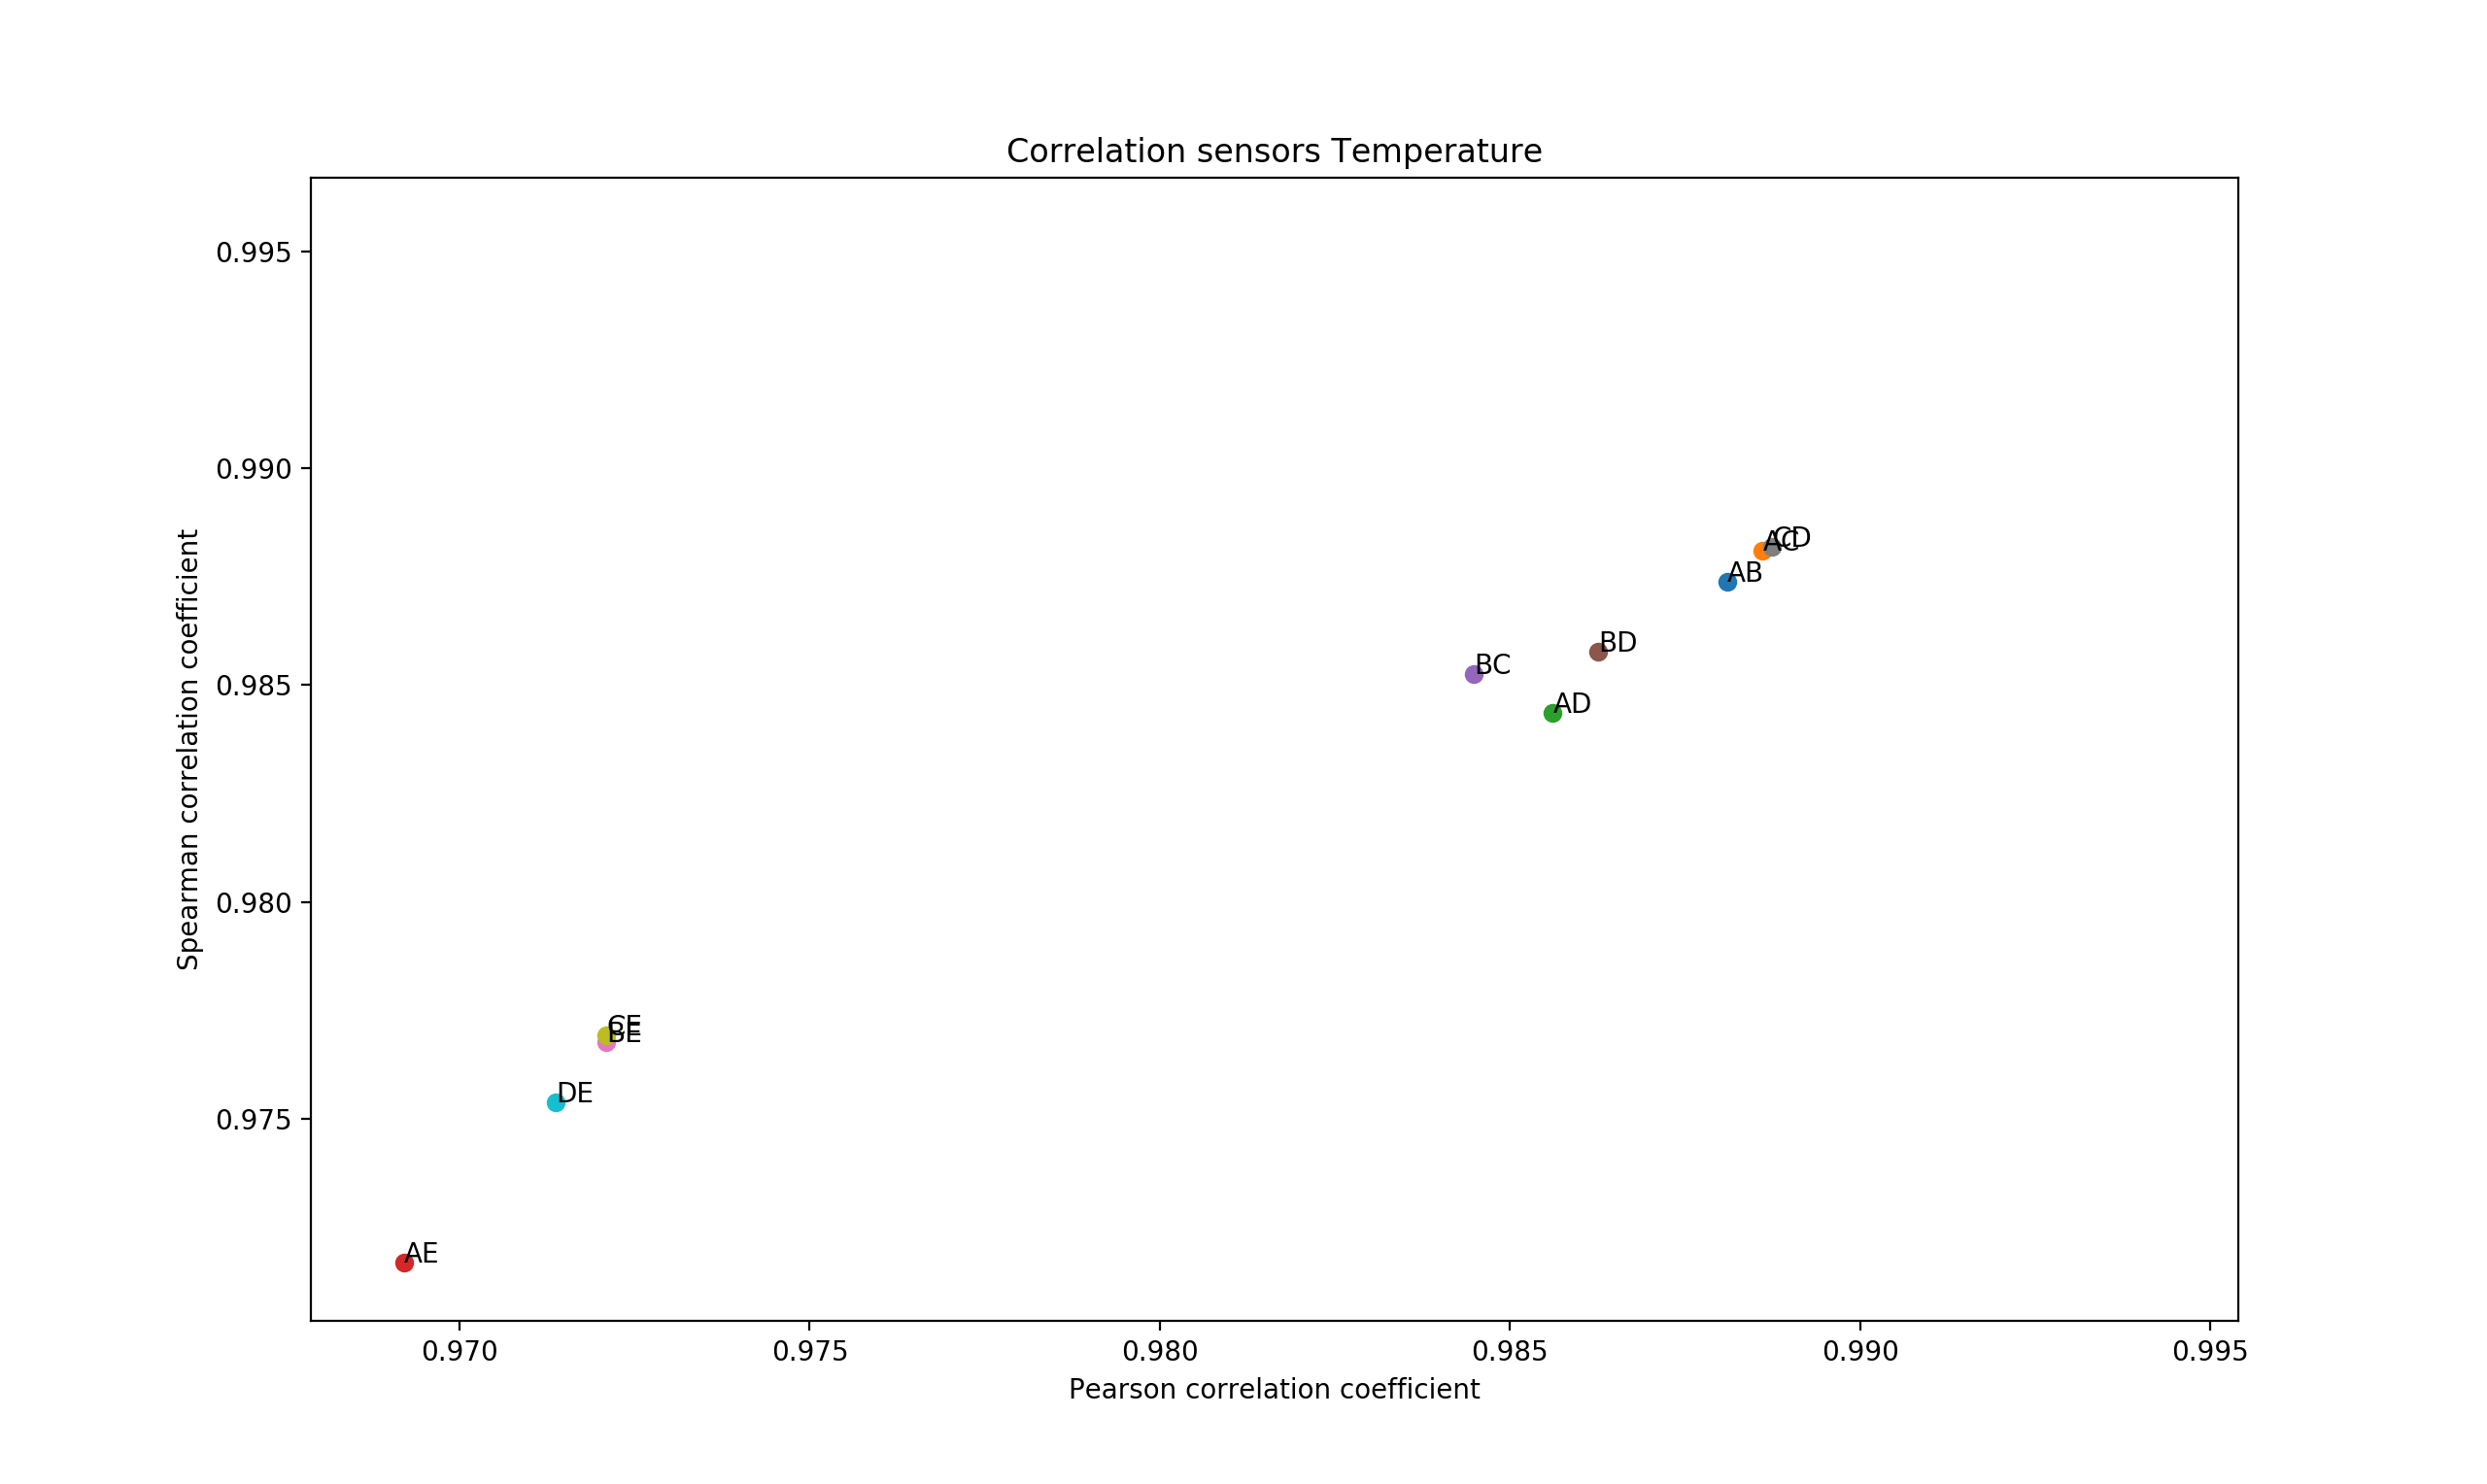
\includegraphics[width=\textwidth]{cor_temp}
        \caption{Spearman and Pearson correlation plot for all sensor combinations of Temperature}
    \end{figure}

    \begin{figure}[H]
        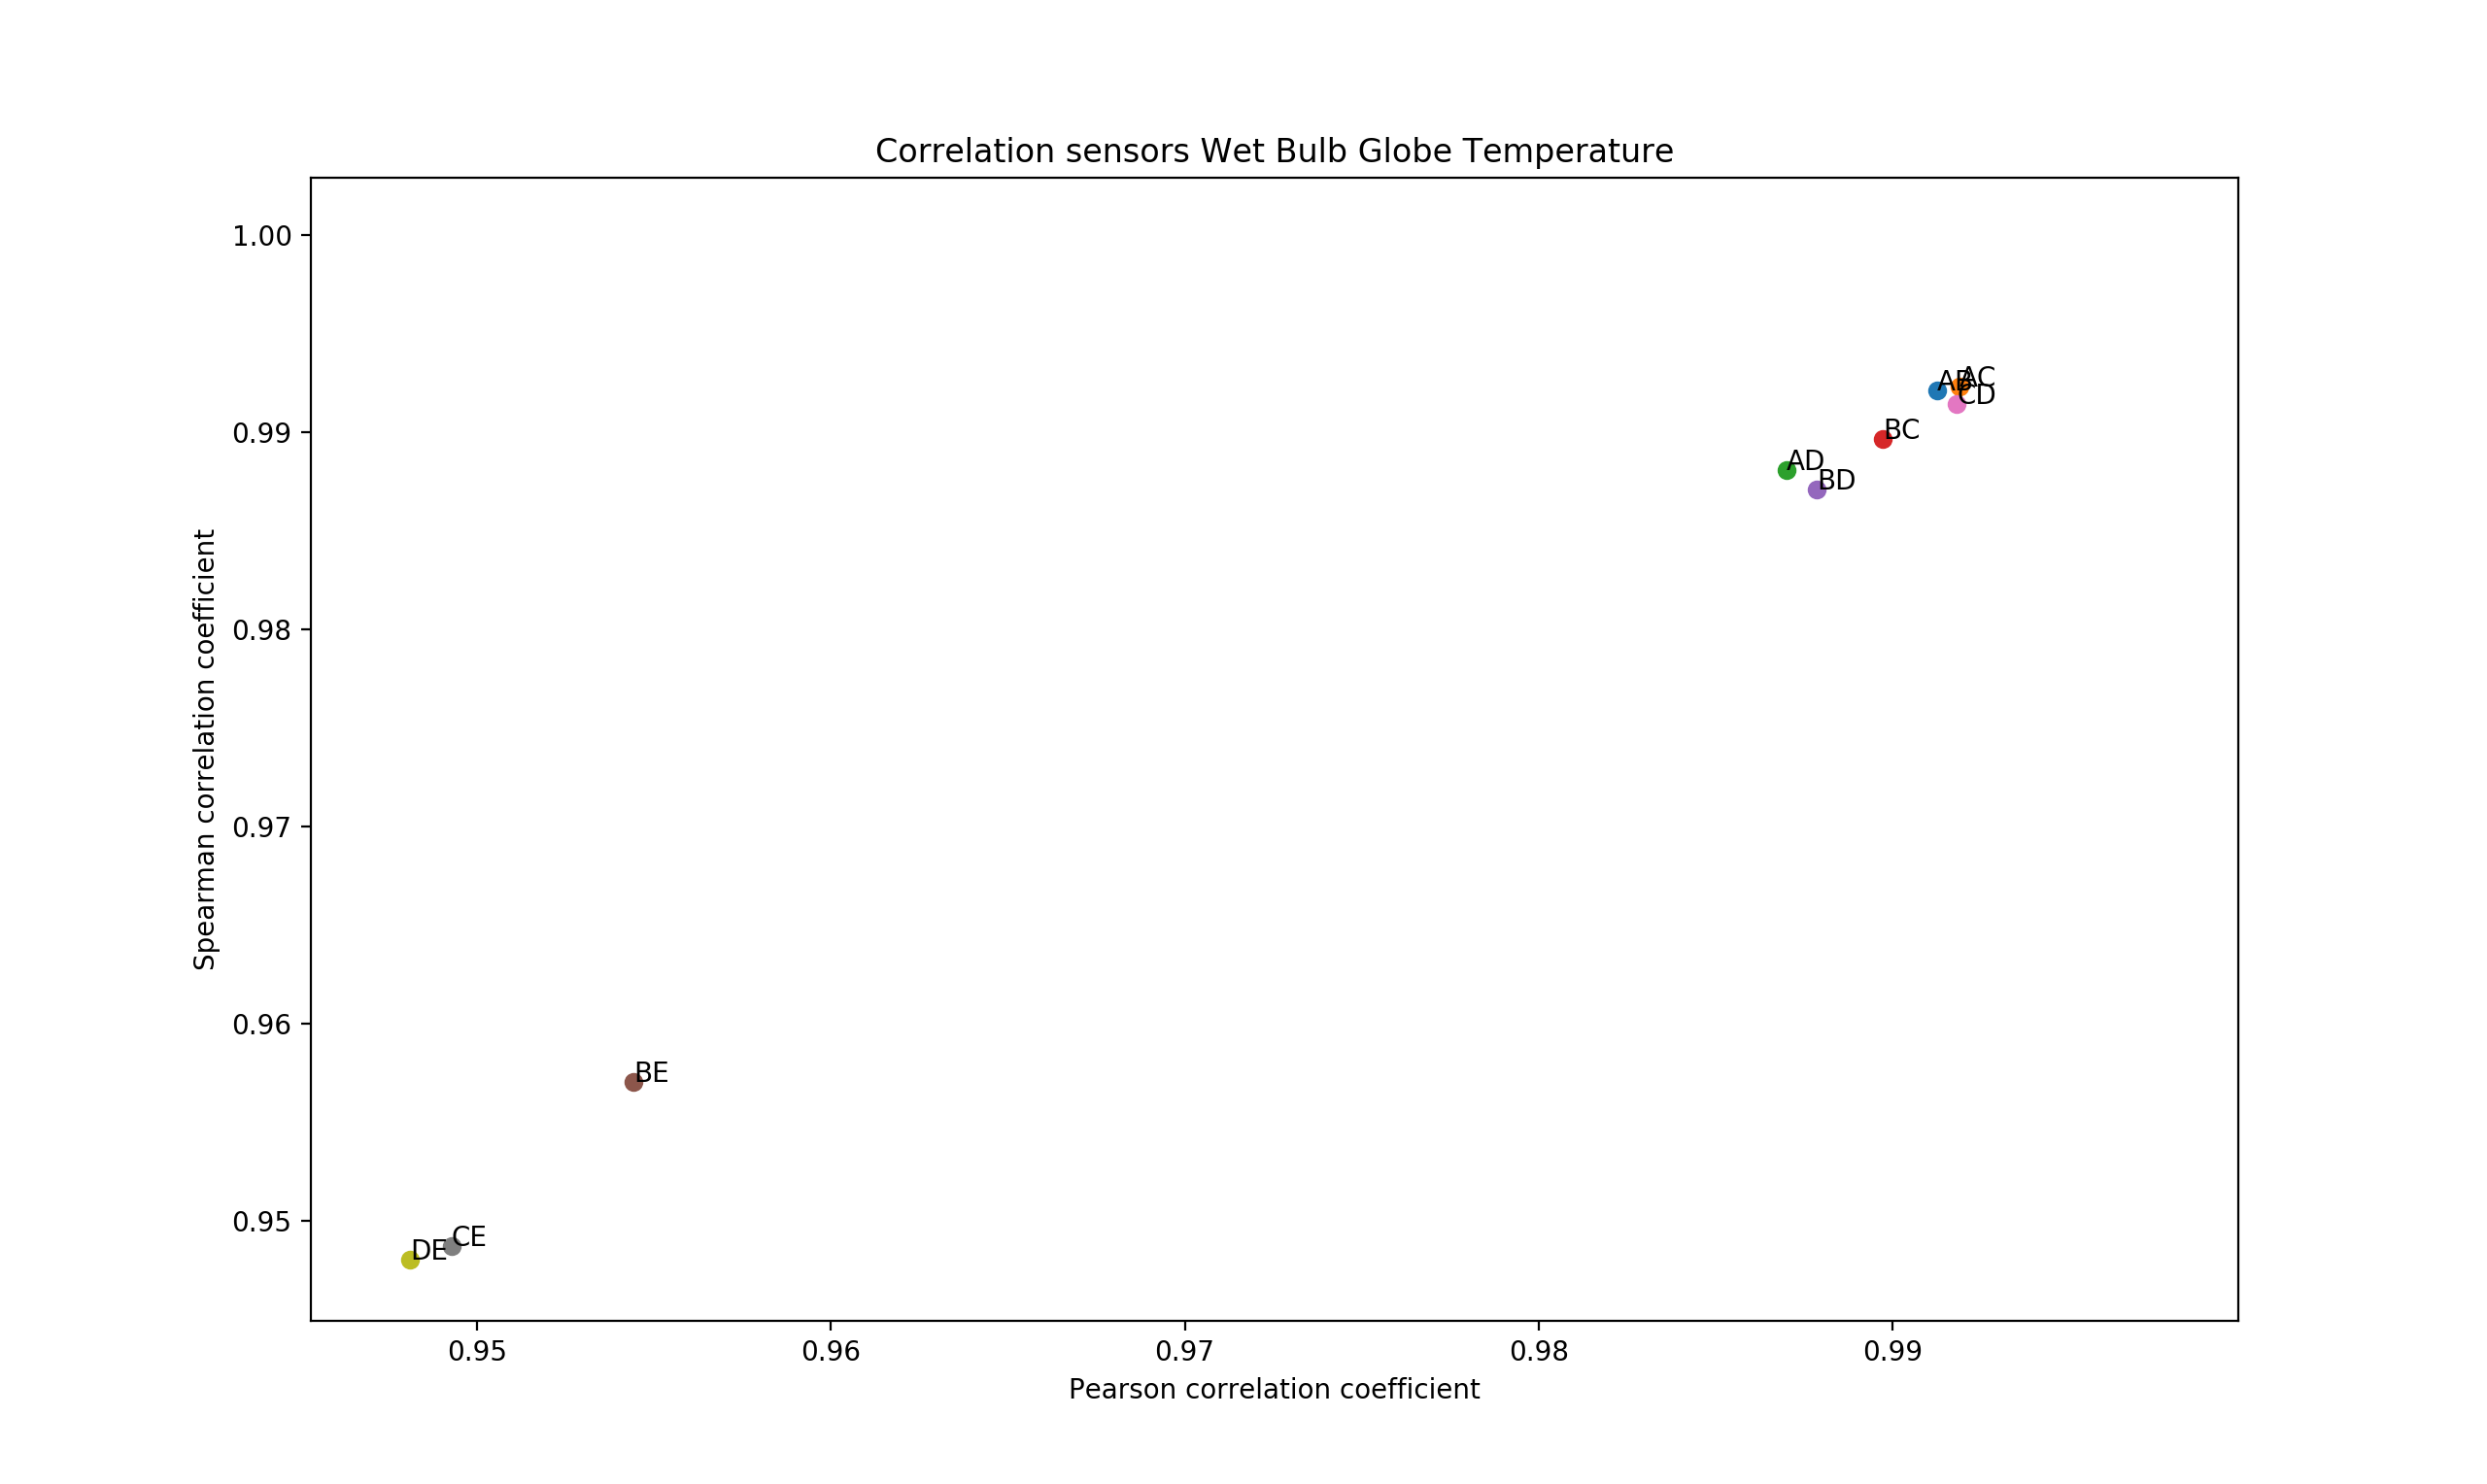
\includegraphics[width=\textwidth]{cor_wbgt}
        \caption{Spearman and Pearson correlation plot for all sensor combinations of Wet Bulb Globe Temperature}
    \end{figure}

    \begin{figure}[H]
        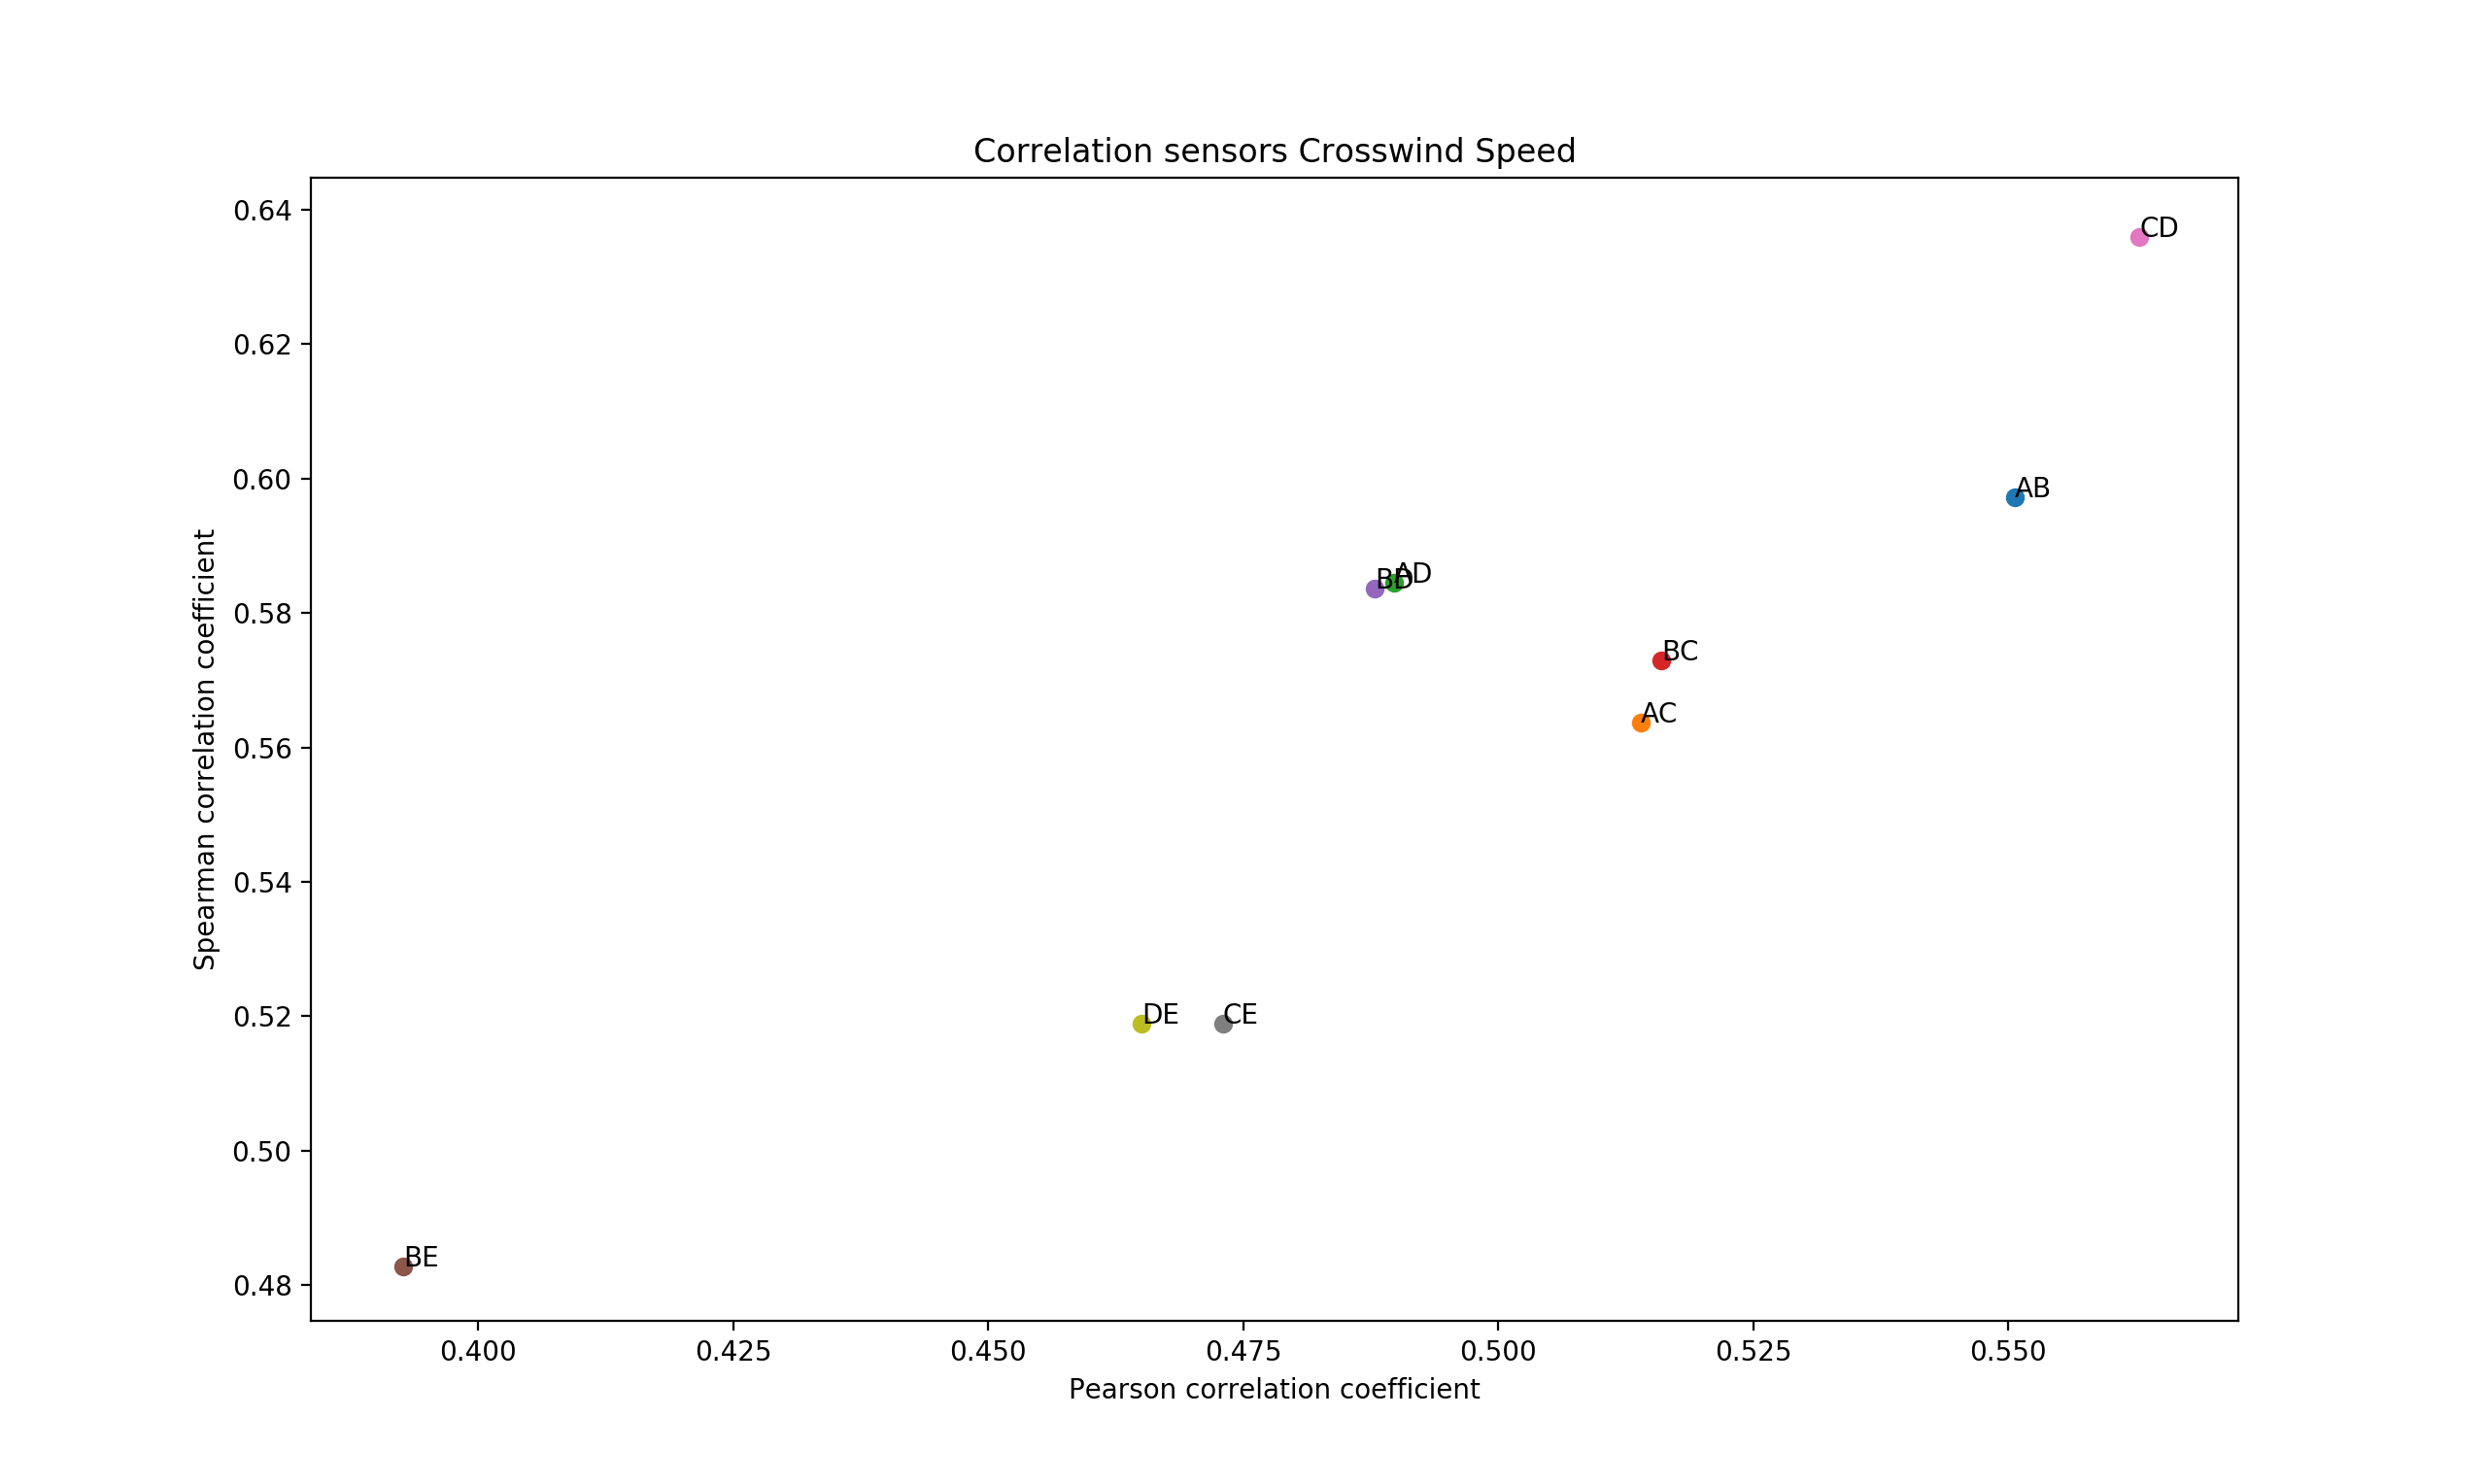
\includegraphics[width=\textwidth]{cor_cwindspeed}
        \caption{Spearman and Pearson correlation plot for all sensor combinations of Crosswind Speed}
    \end{figure}

\section{A4}
    \subsection{Cumulative Density Functions}
        \begin{figure}[H]
            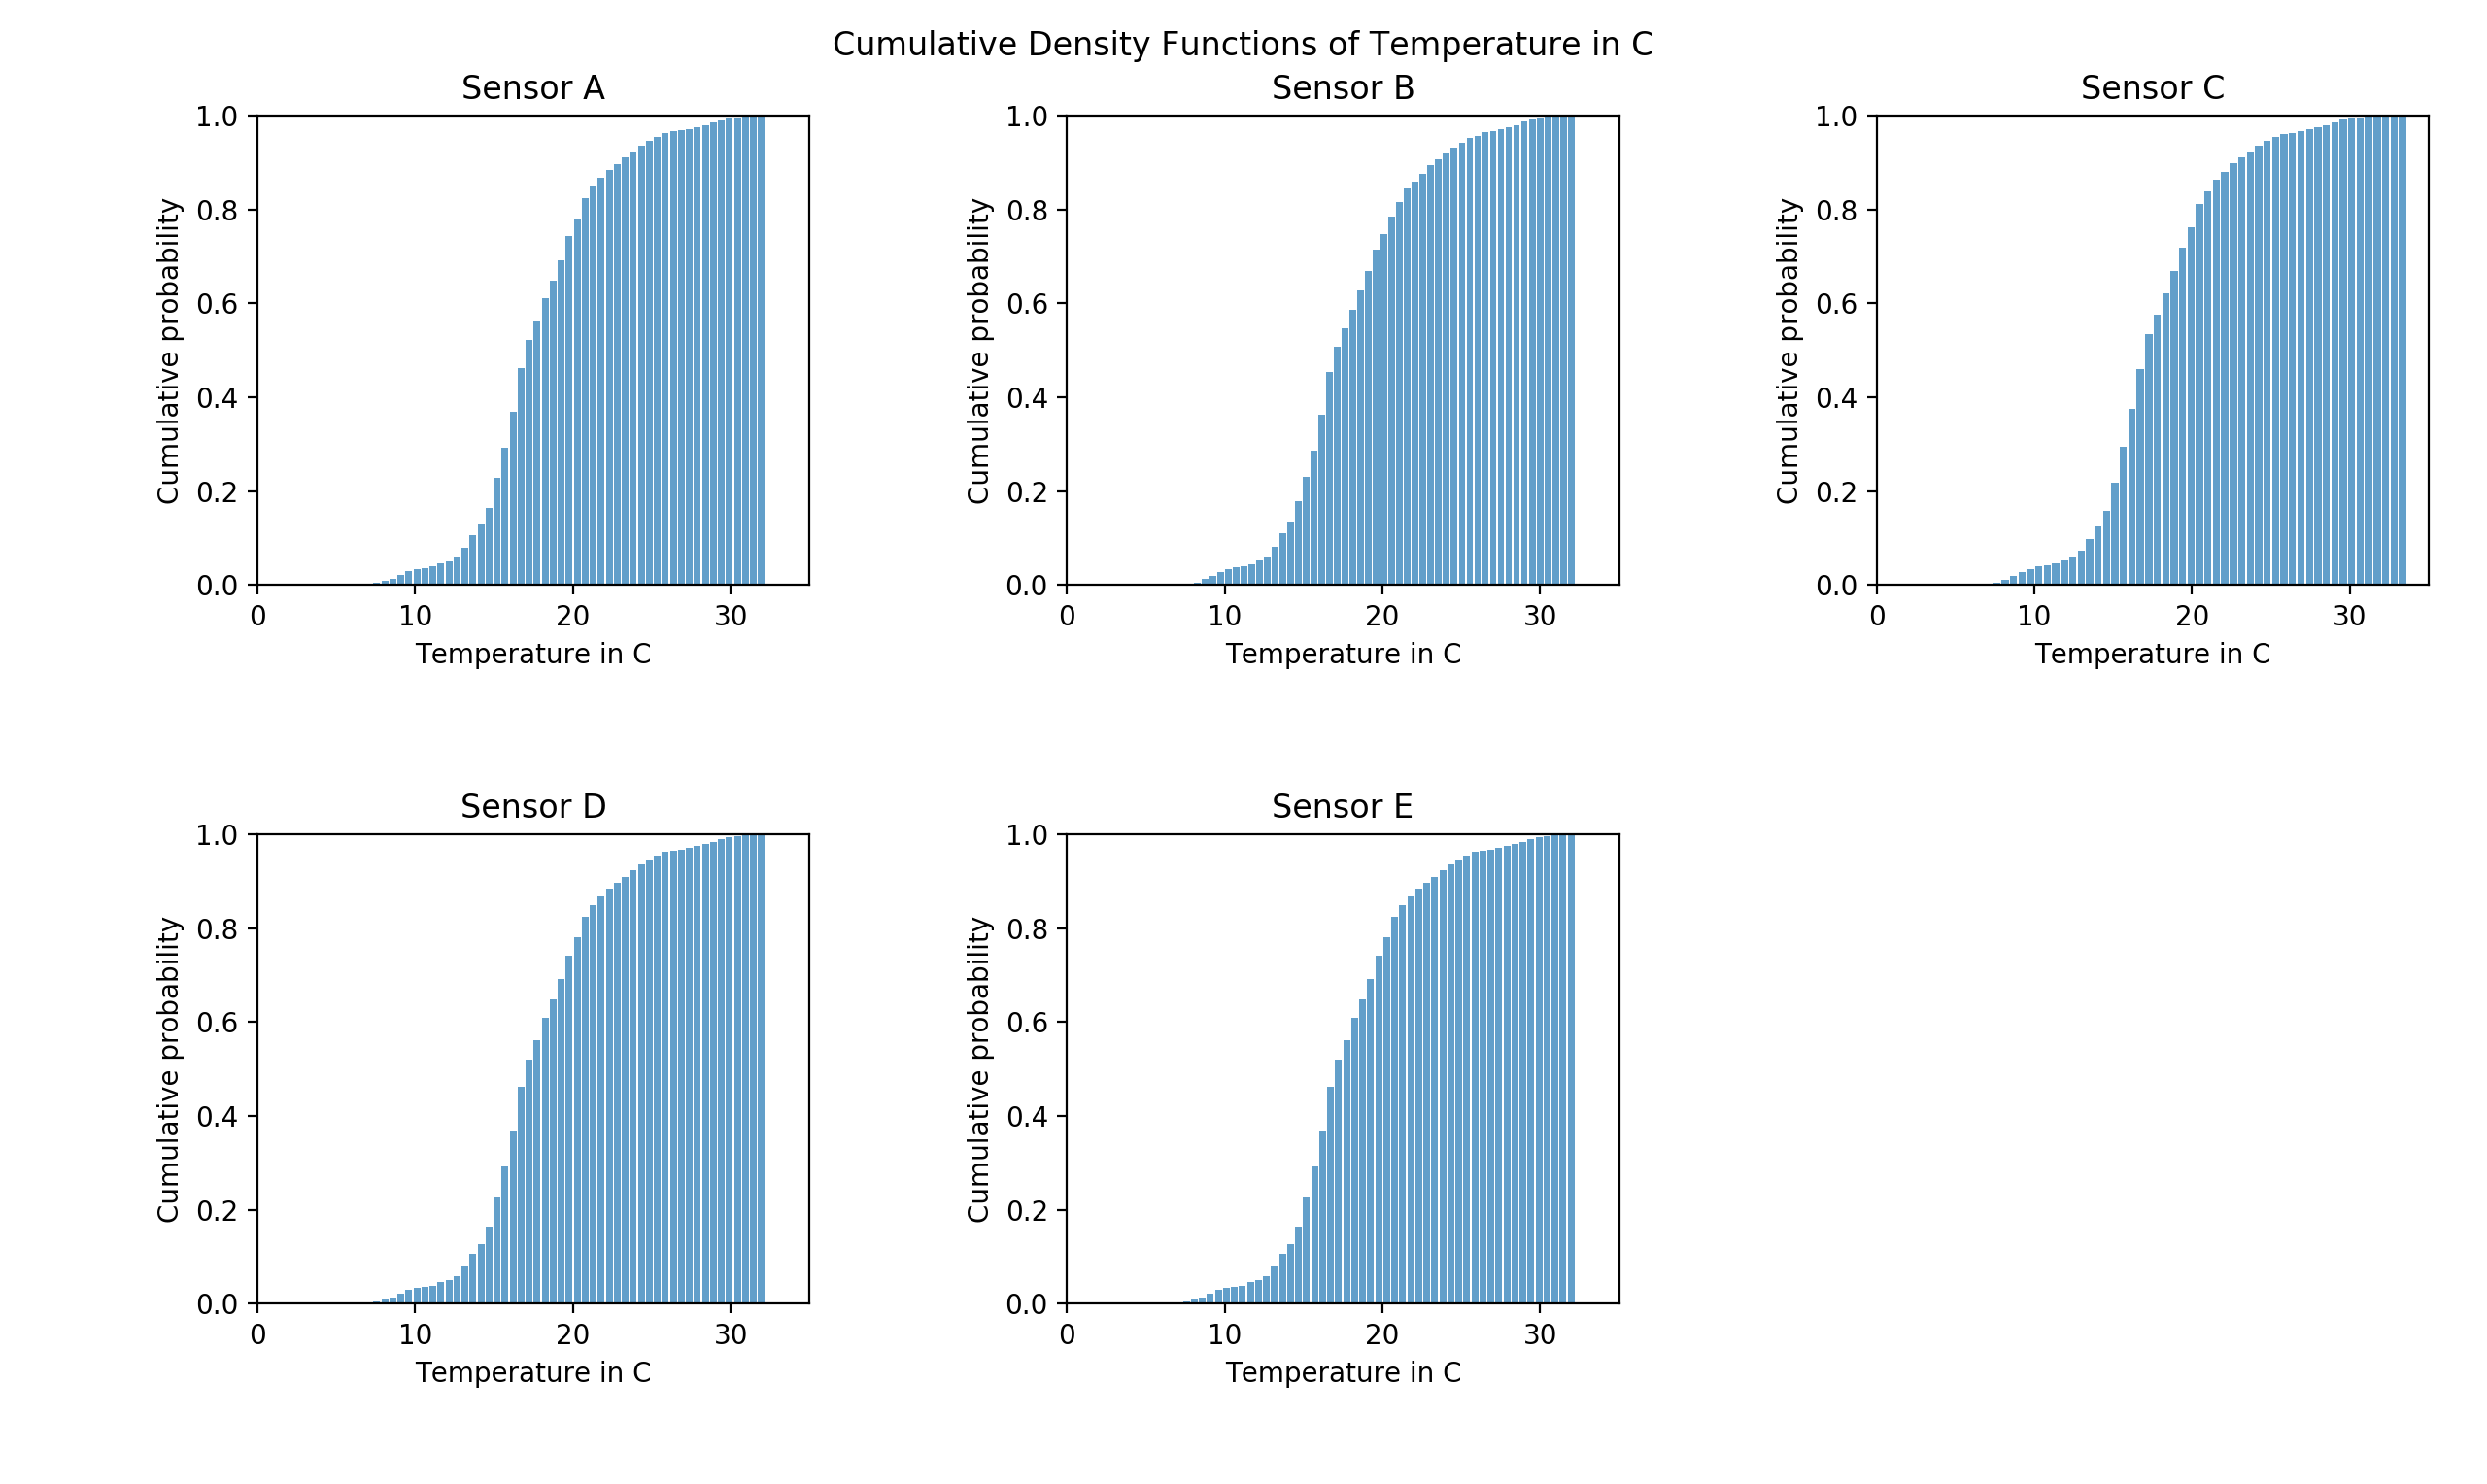
\includegraphics[width=\textwidth]{cdf_temp}
            \caption{Cumilative Density Functions of Temperature for all sensors}
        \end{figure}

        \begin{figure}[H]
            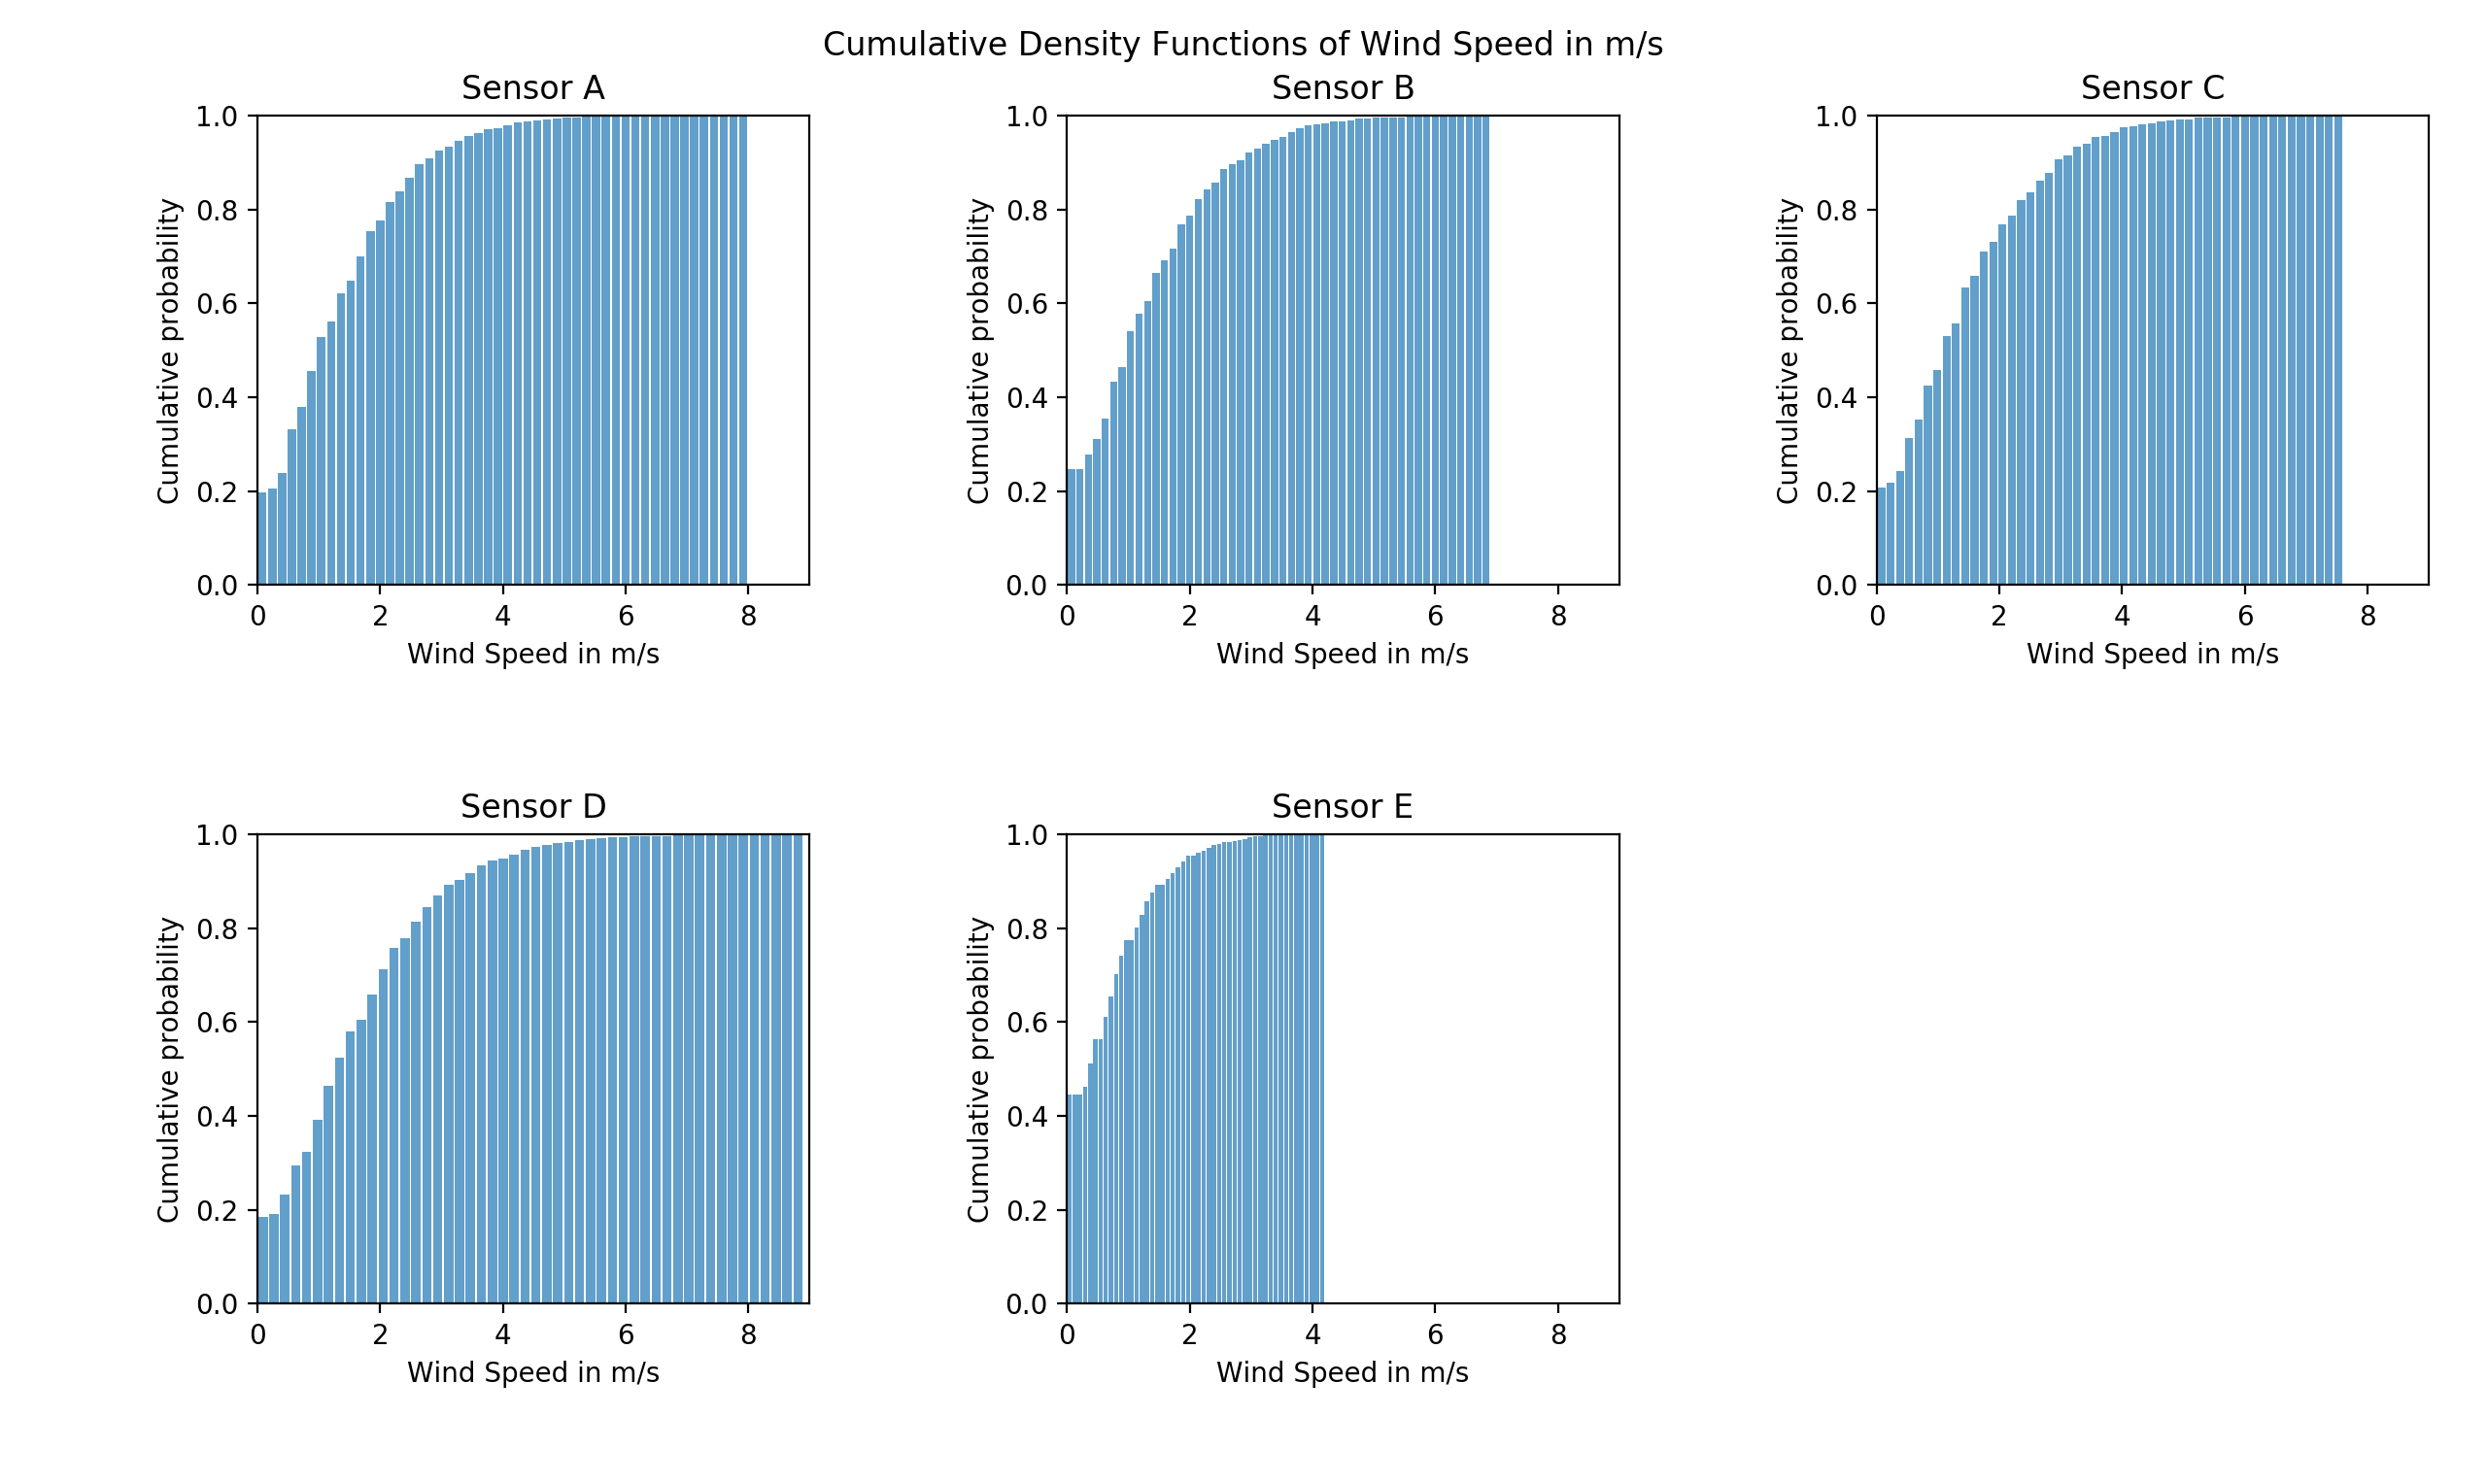
\includegraphics[width=\textwidth]{cdf_windspeed}
            \caption{Cumilative Density Functions of Wind Speed for all sensors}
        \end{figure}

    \subsection{Confidence Intervals}
        \begin{table}[H]
            \caption {Confidence intervals of Temperature for all sensors}
            \begin{tabular}{ll}
            & Temperature                              \\ \hline
            A & (17.81214113267346, 18.126065652463858)  \\
            B & (17.90472689963894, 18.226129320070267)  \\
            C & (17.754926235060246, 18.071347006653575) \\
            D & (17.83814660824381, 18.15457772482005)   \\
            E & (18.181933946027776, 18.525944841851015)
            \end{tabular}
            \end{table}

        \begin{table}[H]
            \caption {Confidence intervals of Wind Speed for all sensors}
            \begin{tabular}{ll}
            & Wind Speed                               \\ \hline
            A & (1.246227038990971, 1.3343868543854427)  \\
            B & (1.1971663346979249, 1.287082453670411)  \\
            C & (1.3243037885948932, 1.418622646328308)  \\
            D & (1.5296480419653757, 1.633650260379006)  \\
            E & (0.5680599051948441, 0.6244249432900044)
            \end{tabular}
            \end{table}

    \subsection{Hypothesis Test}
        \begin{table}[H]
            \caption {Confidence intervals of Wind Speed for all sensors}
            \begin{tabular}{lll}
                        & Temperature             & Wind Speed  \\ \hline
            p-value E, D & 0.0027270117155346967 & 4.899592405994867e-212  \\ 
            p-value C, D & 0.4657972008220813 & 4.610149126224334e-09  \\
            p-value B, C & 0.18562772895626528 & 9.40075204600199e-05  \\
            p-value A, B & 0.40185871871215073 & 0.13247973112544695 
            \end{tabular}
        \end{table}

    \bibliographystyle{plain}
    \bibliography{references.bib}   

\end{document}